% !TEX program = xelatex
% ============================================================================
% មគ្គុទ្ទេសក៍គរុកោសល្យគ្រូ និងរបាយការណ៍ស្រាវជ្រាវលម្អិត (Teacher's Guideline -- EXP412)
% មុខវិជ្ជា៖ គណិតវិទ្យា ថ្នាក់ទី៨ (ពីជគណិត) -- មេរៀនទី២៖ ស្វ័យគុណ
% ចំណុចរង៖ ២.៤.១ ស្វ័យគុណនៃស្វ័យគុណ និង ២.៤.២ ស្វ័យគុណនៃផលគុណ (ទំ.១៧--១៨ ដើម, ២៥--២៦)
% គ្រូបង្រៀន៖ ហុក ប៊ុនថែន | អនុវិទ្យាល័យព្រះក្រសាំង (កំពង់ស្វាយ-កំពង់ធំ)
% ============================================================================
\documentclass[a4paper,12pt]{article}

\usepackage[a4paper, left=1.45cm, right=1.45cm, top=2.30cm, bottom=2.30cm, headheight=18pt, headsep=0.68cm, footskip=0.88cm]{geometry}
\usepackage{amsmath, amssymb}
\usepackage{unicode-math}
\usepackage{fontspec}
\usepackage{array, longtable, multirow, colortbl, booktabs}
\usepackage[table]{xcolor}
\usepackage{enumitem}
\usepackage{pifont}
\usepackage{fancyhdr}
\usepackage{lastpage}
\usepackage{needspace}
\usepackage[hyphens]{url}
\usepackage{tikz}
\usepackage[most]{tcolorbox}
\tcbuselibrary{breakable,skins}
\usetikzlibrary{calc, arrows.meta, positioning, decorations.pathreplacing, decorations.markings, patterns, babel}
\urlstyle{same}

\makeatletter
\let\@expl@@@mark@update@singlecol@structures@@\relax
\makeatother

% ============================================================================
% ការកំណត់ពុម្ពអក្សរផ្លូវការ (Cross-Platform Khmer + Times New Roman APA + Cambria Math)
% ============================================================================
\providecommand{\NGSFindFonts}{%
  \IfFileExists{C:/Windows/Fonts/cambria.ttc}{%
    \def\NGSSysPath{C:/Windows/Fonts/}%
    \def\NGSUserPath{C:/Users/KIT/AppData/Local/Microsoft/Windows/Fonts/}%
  }{%
    \IfFileExists{./fonts/KhmerOSsiemreap.ttf}{\def\NGSSysPath{./fonts/}\def\NGSUserPath{./fonts/}}{%
    \IfFileExists{../fonts/KhmerOSsiemreap.ttf}{\def\NGSSysPath{../fonts/}\def\NGSUserPath{../fonts/}}{%
    \IfFileExists{../../fonts/KhmerOSsiemreap.ttf}{\def\NGSSysPath{../../fonts/}\def\NGSUserPath{../../fonts/}}{%
    \IfFileExists{../../../fonts/KhmerOSsiemreap.ttf}{\def\NGSSysPath{../../../fonts/}\def\NGSUserPath{../../../fonts/}}{%
    \IfFileExists{../../../../fonts/KhmerOSsiemreap.ttf}{\def\NGSSysPath{../../../../fonts/}\def\NGSUserPath{../../../../fonts/}}{%
    \IfFileExists{../../../../../fonts/KhmerOSsiemreap.ttf}{\def\NGSSysPath{../../../../../fonts/}\def\NGSUserPath{../../../../../fonts/}}{%
    \IfFileExists{../../../../../../fonts/KhmerOSsiemreap.ttf}{\def\NGSSysPath{../../../../../../fonts/}\def\NGSUserPath{../../../../../../fonts/}}{%
      \def\NGSSysPath{../../../../../../../fonts/}\def\NGSUserPath{../../../../../../../fonts/}%
    }}}}}}}%
  }%
}
\NGSFindFonts

\setmathfont[
  Path={\NGSSysPath},
  FontIndex=1,
  Scale=1.06
]{cambria.ttc}

\defaultfontfeatures{Ligatures=TeX}

\setmainfont[
  Path={\NGSUserPath},
  Extension=.ttf,
  Script=Khmer,
  BoldFont={KhmerOSsiemreap},
  BoldFeatures={FakeBold=1.8},
  ItalicFont={KhmerOSsiemreap},
  ItalicFeatures={FakeSlant=0.25},
  BoldItalicFont={KhmerOSsiemreap},
  BoldItalicFeatures={FakeBold=1.8, FakeSlant=0.25}
]{KhmerOSsiemreap}

% ហាមដាក់ FakeBold លើ KhmerOSmuollight និងកុំរុំ \muol ក្នុង \textbf{...}
% រាល់អក្សរឡាតាំង លេខ ឬសញ្ញា ASCII ក្នុង \muol ត្រូវរុំក្នុង \enbf{...} ឬ $...$
\newfontfamily\muol[
  Path={\NGSUserPath},
  Extension=.ttf,
  Script=Khmer
]{KhmerOSmuollight}

\newfontfamily\TimesEn[
  Path={\NGSSysPath},
  Extension=.ttf,
  Scale=1.02,
  BoldFont={timesbd},
  ItalicFont={timesi},
  BoldItalicFont={timesbi}
]{times}

\newfontfamily\Tacteing[
  Path={\NGSUserPath}
]{TACTENG.TTF}

\newfontfamily\CourierBullet[
  Path={\NGSSysPath},
  Extension=.ttf
]{cour}

% ក្បួនកាត់ពាក្យខ្មែរ (Khmer word wrapping)
\XeTeXlinebreaklocale "km"
\XeTeXlinebreakskip = 0pt plus 1pt minus 0.1pt

% Mobile-First spacing (11.5pt / 18.2pt exact)
\linespread{1.0}

% ============================================================================
% ពណ៌ ស-ខ្មៅ (Strict Monochrome Grayscale Palette) & Fancyhdr
% ============================================================================
\definecolor{headgray}{HTML}{F2F2F2}
\definecolor{panelgray}{gray}{0.94}
\definecolor{stepgray}{HTML}{D9D9D9}
\definecolor{midgray}{gray}{0.82}
\definecolor{bordergray}{gray}{0.45}

\pagestyle{fancy}
\fancyhf{}
\renewcommand{\headrulewidth}{0.4pt}
\renewcommand{\footrulewidth}{0.4pt}
\fancyhead[L]{\rule[-3pt]{0pt}{14pt}\fontsize{9.5pt}{13pt}\selectfont មគ្គុទ្ទេសក៍គរុកោសល្យគ្រូ \en{(Grade 8 EXP412)}}
\fancyhead[R]{\rule[-3pt]{0pt}{14pt}\fontsize{9.5pt}{13pt}\selectfont មេរៀនទី២ \en{(}២.៤.១--២.៤.២\en{)}៖ ស្វ័យគុណនៃស្វ័យគុណ និងផលគុណ}
\fancyfoot[L]{\rule{0pt}{13pt}\fontsize{9.5pt}{13pt}\selectfont កញ្ចប់ឯកសារ \en{NGS 5Es (}៥០ នាទី\en{) |} ហុក ប៊ុនថែន}
\fancyfoot[R]{\rule{0pt}{13pt}\fontsize{9.5pt}{13pt}\selectfont ទំព័រ \en{\thepage\ / \pageref{LastPage}}}

\fancypagestyle{firstpage}{%
  \fancyhf{}%
  \renewcommand{\headrulewidth}{0pt}%
  \renewcommand{\footrulewidth}{0.4pt}%
  \fancyfoot[L]{\rule{0pt}{13pt}\fontsize{9.5pt}{13pt}\selectfont កញ្ចប់ឯកសារ \en{NGS 5Es (}៥០ នាទី\en{) |} អនុវិទ្យាល័យព្រះក្រសាំង}%
  \fancyfoot[R]{\rule{0pt}{13pt}\fontsize{9.5pt}{13pt}\selectfont ទំព័រ \en{\thepage\ / \pageref{LastPage}}}%
}

\setlength{\parindent}{0pt}
\setlength{\parskip}{4.5pt}
\setlength{\tabcolsep}{4pt}
\setlength{\emergencystretch}{2em}
\setlist{itemsep=2.8pt, parsep=0pt}

% ============================================================================
% ម៉ាក្រូជំនួយ និងឋានានុក្រម \muol គ្មានតួអក្សរ ASCII បន្លំ
% ============================================================================
\newcommand{\en}[1]{{\TimesEn #1}}
\newcommand{\enbf}[1]{{\TimesEn\textbf{#1}}}
\newcommand{\enit}[1]{{\TimesEn\textit{#1}}}
\newcommand{\unit}[1]{\,\text{\en{#1}}}
\newcommand{\cnum}[1]{{\TimesEn\fontsize{10.5pt}{12pt}\selectfont\ding{\numexpr181+#1\relax}}}
\newcommand{\ditem}{\tikz[baseline=-0.5ex]\fill (0,0.40ex) -- (0.40ex,0) -- (0,-0.40ex) -- (-0.40ex,0) -- cycle;\hspace{0.25em}}
\newcommand{\wcirc}{{\CourierBullet\fontsize{9.8pt}{11pt}\selectfont o}}
\newcommand{\chkbox}{\tikz[baseline=-0.15ex]\draw[black, line width=0.85pt] (0,0) rectangle (0.25cm,0.25cm);}
\newcommand{\khmflourish}{{\Tacteing\fontsize{38pt}{15pt}\selectfont\raisebox{-5pt}{3}}}

\newcommand{\parttitle}[1]{{\muol\fontsize{14pt}{22pt}\selectfont #1}}
\newcommand{\sectitle}[1]{{\muol\fontsize{12pt}{19pt}\selectfont #1}}
\newcommand{\subsectitle}[1]{{\muol\fontsize{11.5pt}{18.5pt}\selectfont #1}}
\newcommand{\tblhead}[1]{{\muol\fontsize{10.2pt}{16pt}\selectfont #1\par}}
\newcommand{\teachersays}[1]{{\muol\fontsize{10.8pt}{17pt}\selectfont «គ្រូនិយាយថា៖} #1»}

\newcolumntype{L}[1]{>{\raggedright\arraybackslash}p{#1}}
\newcolumntype{C}[1]{>{\centering\arraybackslash}p{#1}}
\newcolumntype{R}[1]{>{\raggedleft\arraybackslash}p{#1}}

\newcommand{\secbanner}[2]{%
  \Needspace{2.2cm}%
  \vspace{2pt}%
  \begin{tcolorbox}[
    enhanced, sharp corners, colback=stepgray, colframe=black,
    boxrule=1.1pt, borderline south={0.6pt}{1.8pt}{black},
    top=6pt, bottom=6pt, left=9pt, right=9pt,
    before skip=4pt, after skip=4pt
  ]
    \sectitle{#1}\\[2pt]
    {\fontsize{10pt}{14.5pt}\selectfont\enit{#2}}%
  \end{tcolorbox}%
}

\newcommand{\refbanner}[1]{%
  \Needspace{2.2cm}%
  \vspace{2pt}%
  \begin{tcolorbox}[
    enhanced, sharp corners, colback=headgray, colframe=black,
    boxrule=0.85pt, borderline south={0.6pt}{1.8pt}{black},
    top=6pt, bottom=6pt, left=9pt, right=9pt,
    before skip=4pt, after skip=4pt
  ]
    {\muol\fontsize{12pt}{19pt}\selectfont #1}%
  \end{tcolorbox}%
}

\newcommand{\subsec}[1]{%
  \Needspace{1.7cm}%
  \vspace{3pt}%
  \subsectitle{#1}\par%
  \vspace{-2pt}%
  {\color{black}\hrule height 0.55pt}%
  \vspace{3pt}%
}

\newtcolorbox{phasebox}[3]{%
  enhanced, breakable, sharp corners,
  colback=white, colframe=black,
  boxrule=1.0pt, top=5pt, bottom=5pt, left=9pt, right=9pt,
  toptitle=3.5pt, bottomtitle=3.5pt,
  before skip=5pt, after skip=0pt,
  colbacktitle=headgray, coltitle=black,
  fonttitle=\fontsize{11pt}{17.5pt}\selectfont,
  fontupper=\fontsize{11.5pt}{18.2pt}\selectfont,
  title={%
    \linespread{1.0}\selectfont\renewcommand{\arraystretch}{1.0}%
    \begin{tabular*}{\linewidth}{@{}>{\raggedright\arraybackslash}p{13.55cm}@{\extracolsep{\fill}}r@{}}
      {\muol\fontsize{11pt}{17.5pt}\selectfont #1} & {\fontsize{10.5pt}{15pt}\selectfont\en{#2 |} #3}%
    \end{tabular*}%
  }
}

\newtcolorbox{scriptbox}{%
  enhanced, breakable, sharp corners, colback=panelgray, colframe=black,
  boxrule=0.8pt, borderline west={2.4pt}{0pt}{black},
  top=5pt, bottom=5pt, left=9pt, right=8pt,
  before skip=-0.5pt, after skip=5pt,
  fontupper=\fontsize{11.5pt}{18.2pt}\selectfont
}

\begin{document}
\thispagestyle{firstpage}
\fontsize{11.5pt}{18.2pt}\selectfont
\vspace*{-0.75cm}

% ============================================================================
% ក្បាលលិខិតផ្លូវការថ្នាក់ជាតិ & សាលារៀន (Kampong Thom / Kampong Svay / Preah Krasang)
% ============================================================================
{\linespread{1.08}\selectfont
\begin{center}
  {\muol\fontsize{13.5pt}{21pt}\selectfont ព្រះរាជាណាចក្រកម្ពុជា}\\[2pt]
  {\muol\fontsize{12pt}{18.5pt}\selectfont ជាតិ សាសនា ព្រះមហាក្សត្រ}\\[1pt]
  \khmflourish
\end{center}
\vspace{-4pt}
{\muol\fontsize{10.8pt}{17pt}\selectfont
  មន្ទីរអប់រំ យុវជន និងកីឡា ខេត្តកំពង់ធំ\\
  ការិយាល័យអប់រំ យុវជន និងកីឡា ស្រុកកំពង់ស្វាយ\\
  អនុវិទ្យាល័យព្រះក្រសាំង\par}
\vspace{4pt}
\begin{center}
  \parttitle{មគ្គុទ្ទេសក៍គរុកោសល្យគ្រូ និងរបាយការណ៍ស្រាវជ្រាវ \enbf{(Teacher's Guideline)}}\\[3pt]
  {\fontsize{11.5pt}{18pt}\selectfont\textbf{គណិតវិទ្យា ថ្នាក់ទី៨ \en{(}ពីជគណិត\en{)} \en{---} មេរៀនទី២៖ ស្វ័យគុណ}}\\
  {\fontsize{11.0pt}{17pt}\selectfont\textbf{២.៤.១ ស្វ័យគុណនៃស្វ័យគុណ និង ២.៤.២ ស្វ័យគុណនៃផលគុណ \en{(}ទំព័រ ១៧--១៨ ដើម\en{)}}}
\end{center}
}

\vspace{2pt}
\begin{tcolorbox}[
  enhanced, breakable, sharp corners, colback=headgray, colframe=black,
  boxrule=0.85pt, top=5pt, bottom=5pt, left=7pt, right=7pt,
  before skip=2pt, after skip=5pt
]
  {\muol\fontsize{11pt}{17pt}\selectfont ព័ត៌មានរដ្ឋបាលមេរៀន \enbf{(Lesson Package Metadata)}}\par\vspace{3pt}
  \linespread{1.0}\fontsize{10.5pt}{15pt}\selectfont
  \renewcommand{\arraystretch}{1.15}
  \begin{tabular}{@{}L{2.85cm}@{}C{0.25cm}@{}L{5.25cm}@{\hspace{0.25cm}}L{2.50cm}@{}C{0.25cm}@{}L{5.65cm}@{}}
    \textbf{\en{-} មុខវិជ្ជា \en{/} ថ្នាក់} & \en{:} & គណិតវិទ្យា ថ្នាក់ទី៨ \en{(}ពីជគណិត\en{)} & \textbf{\en{-} កាលបរិច្ឆេទ} & \en{:} & \makebox[28mm]{\dotfill}\ ២០២៦ \en{(}ព.ស. ២៥៧០\en{)} \\
    \textbf{\en{-} មេរៀន \en{/} ផ្នែក} & \en{:} & មេរៀនទី២៖ ស្វ័យគុណ \en{(2.4.1--2.4.2)} & \textbf{\en{-} រយៈពេល} & \en{:} & ៥០ នាទី \en{(}១ ម៉ោងសិក្សា\en{)} \\
    \textbf{\en{-} សៀវភៅគោល} & \en{:} & \en{MoEYS} ទំ. ១៧--១៨ ដើម, ២៥--២៦ & \textbf{\en{-} បង្រៀនដោយ} & \en{:} & ហុក ប៊ុនថែន \en{(NGS} ព្រះក្រសាំង\en{)} \\
    \textbf{\en{-} កញ្ចប់ឯកសារ} & \en{:} & \multicolumn{4}{@{}L{13.90cm}@{}}{ឯកសារ \en{LaTeX} ៤ ច្បាប់ \en{(LS\_Plan, Scenario, Guideline, Printable)} + ថតភស្តុតាង \en{15 OA PDFs}}
  \end{tabular}
\end{tcolorbox}

% ============================================================================
% ផ្នែកទី ១៖ បរិបទមេរៀន និងទិដ្ឋភាពទូទៅនៃកញ្ចប់ឯកសារ ៥ ផ្នែក
% ============================================================================
\secbanner{ផ្នែកទី ១៖ បរិបទមេរៀន និងទិដ្ឋភាពទូទៅនៃកញ្ចប់ឯកសារ ៥ ផ្នែក}{Section 1: Administrative Context, MoEYS Textbook Audit (pp. 16--18, 25--26) \& 5-Part Package Synchronization}

\subsec{១\enbf{.}១ បរិបទអនុវិទ្យាល័យព្រះក្រសាំង និងតួនាទីនៃចំណុចរង ២\enbf{.}៤\enbf{.}១\enbf{--}២\enbf{.}៤\enbf{.}២}

ចំណុចរង \textbf{២.៤.១ «ស្វ័យគុណនៃស្វ័យគុណ»} និង \textbf{២.៤.២ «ស្វ័យគុណនៃផលគុណ»} (ទំព័រ ១៧--១៨ ដើម នៃសៀវភៅគណិតវិទ្យា ថ្នាក់ទី៨ ក្រសួងអប់រំ យុវជន និងកីឡា) គឺជាចំណុចបំប្លែងគន្លឹះនៅក្នុងមេរៀនទី២៖ ស្វ័យគុណ។ នៅក្នុងម៉ោងសិក្សាមុនៗ (ចំណុចទី ១--៣ ទំព័រ ១៣--១៦) សិស្សបានរៀនពីនិយមន័យស្វ័យគុណវិជ្ជមាន វិធីគុណស្វ័យគុណគោលដូចគ្នា ($a^m\cdot a^n = a^{m+n}$) និងវិធីចែកស្វ័យគុណ ($\frac{a^m}{a^n} = a^{m-n}$, ស្វ័យគុណសូន្យ $a^0=1$ និងនិទស្សន្តអវិជ្ជមាន $a^{-n}=\frac{1}{a^n}$ ចំពោះ $a\neq 0$)។ មកដល់ចំណុចទី ៤ (\textbf{លក្ខណៈនៃស្វ័យគុណ}) សិស្សត្រូវធ្វើបន្សាំការគិតទៅកាន់ប្រតិបត្តិការពីរជាន់ គឺ \textbf{ស្វ័យគុណលើស្វ័យគុណ} $(a^m)^n = a^{m\cdot n}$ និង \textbf{ស្វ័យគុណចែកចាយលើផលគុណ} $(a\cdot b)^n = a^n \cdot b^n$ ដែលនឹងក្លាយជាមូលដ្ឋានផ្ទាល់សម្រាប់ \textbf{២.៤.៣ ស្វ័យគុណនៃផលចែក} និង \textbf{ទម្រង់ស្តង់ដា} នៅចុងមេរៀន។

តាមរយៈការសង្កេតថ្នាក់រៀនជាក់ស្ដែងនៅ \textbf{អនុវិទ្យាល័យព្រះក្រសាំង (សាលារៀនជំនាន់ថ្មី \en{NGS})} ស្រុកកំពង់ស្វាយ ខេត្តកំពង់ធំ និងការផ្ទៀងផ្ទាត់ទំព័រសៀវភៅសិក្សាគោលដោយផ្ទាល់ (\en{Book pp. 16--18, 25--26}), កញ្ចប់ឯកសារ \en{\_EXP412} ត្រូវបានរចនាឡើងដើម្បីដោះស្រាយបញ្ហាប្រឈមធំៗចំនួន ៤ យ៉ាង៖
\begin{itemize}[leftmargin=0.65cm]
  \item \textbf{១. ភាពច្រឡំប្រមាណវិធីបូកនិងគុណនិទស្សន្ត ($a^m\cdot a^n$ vs $(a^m)^n$)៖} នៅពេលផ្លាស់ប្ដូររហ័សពី $2^3\cdot 2^4 = 2^{3+4} = 2^7$ មក $(2^3)^4$ សិស្សតែងបន្តយក $3+4=7$ ដោយមិនស្គាល់ពីរចនាសម្ព័ន្ធ «៤ ក្រុមនៃ ៣ កត្តា»។ ម៉្យាងទៀត នៅក្នុងប្រអប់ \textbf{«ជាទូទៅ ៤.១ និង ៤.២» (ទំ.១៧)} សៀវភៅចែងត្រឹម \textit{«$a, b$ ជាចំនួនសនិទាន និង $m, n$ ជាចំនួនគត់រ៉ឺឡាទីបខុសពីសូន្យ»} ដោយពុំបានរំលឹកលក្ខខណ្ឌ \textbf{$a\neq 0, b\neq 0$} ពេលនិទស្សន្តជាចំនួនអវិជ្ជមានឡើយ។
  \item \textbf{២. អន្ទាក់លីនេអ៊ែរលើផលបូក \en{(Freshman's Dream)} និងការភ្លេចមេគុណ៖} សិស្សងាយពង្រីកខុស $(3b)^2 = 3b^2$, $(3xy^2)^3 = 3x^3y^6$ (ភ្លេចលើកស្វ័យគុណមេគុណលេខ $3$) ឬច្រឡំអនុវត្តលក្ខណៈផលគុណទៅលើផលបូកដូចជា $(2+3)^2 = 2^2+3^2$។
  \item \textbf{៣. វិសាលភាពសញ្ញាដកនិងវង់ក្រចក៖} ក្នុងលំហាត់ \textbf{ប្រតិបត្តិ ៤.២ ក (ទំ.១៨)} គឺ $-2(a^{-3}\cdot b^5)^2$ សិស្សងាយច្រឡំយក $-2$ ទៅលើកស្វ័យគុណ $2$ ជាមួយវង់ក្រចកដូច $(-2x^3y)^2$ ហើយបាត់សញ្ញាដកមុខលទ្ធផល $-\frac{2b^{10}}{a^6}$។
  \item \textbf{៤. ការផ្ទៀងផ្ទាត់ពុម្ពសៀវភៅគោល (ទំ.១៧, ១៨ និង ២៦)៖} ការពិនិត្យសៀវភៅគោលរកឃើញថា នៅ \textbf{ទំ.១៧} ឧទាហរណ៍ ៤.២ (ក, ខ) ខ្វះសញ្ញាខណ្ឌ «។» ចុងល្បះ និង \textbf{ទំ.២៦} \en{\#8}គ ខ្វះសញ្ញាចុច «.» ក្រោយអក្សរ «គ»។ អ្វីដែលគ្រូត្រូវយកចិត្តទុកដាក់បំផុតគឺ \textbf{ទំ.១៨ ប្រតិបត្តិ ខ.} បោះពុម្ពថា \textbf{$a \cdot (a^4) \cdot a^{-6}$} (គ្មាននិទស្សន្ត $5$ ខាងក្រៅវង់ក្រចក) ខុសពី \textbf{ទំ.១៧ ប្រតិបត្តិ ខ.} ដែលបោះពុម្ពថា \textbf{$a \cdot (a^4)^5 \cdot a^{-6}$}។ ប្រសិនបើសិស្សមិនអានវង់ក្រចកដោយប្រុងប្រយ័ត្នទេ ពួកគេនឹងស្មានយកចម្លើយ $a^{15}$ មកដាក់ជំនួស $\frac{1}{a}$ ដោយច្រឡំ។
\end{itemize}

\subsec{១\enbf{.}២ សមាហរណកម្មកញ្ចប់ឯកសារ ៥ ផ្នែក និងផែនទីភស្តុតាង}

ឯកសារទាំង ៤ ក្នុងថតមេរៀន ២.៤.១\_២.៤.២ រួមជាមួយថតភស្តុតាង \en{PDF} ត្រូវបានរៀបចំឱ្យស៊ីចង្វាក់គ្នា ១០០\% ទាំងលេខលំហាត់ វង់ក្រចក \en{B\&W} ធនាគារហេតុផល \cnum{1}--\cnum{5} និងពាក្យពេចន៍ក្នុងកាតសិស្ស៖
\begin{enumerate}[leftmargin=0.65cm]
  \item \textbf{\en{LS\_Plan\_EXP412.tex/.pdf}}៖ កិច្ចតែងការបង្រៀន ៥០ នាទី គំរូ \en{5Es} (\en{2 + 9 + 17 + 20 + $\le$2 min}) សរសេរជាជួររងតូចៗងាយអានសម្រាប់គ្រូប្រើប្រាស់ផ្ទាល់ក្នុងថ្នាក់។
  \item \textbf{\en{Teaching\_Scenario\_EXP412.tex/.pdf}}៖ សេណារីយ៉ូគ្រប់គ្រងនាទី-ទល់-នាទី ការផ្ទេរសម្ភារៈ ៣ តួនាទី ប្លង់ក្ដារខៀន ៣ ផ្នែក និងតារាងកំហុសជាក់ស្ដែង។
  \item \textbf{\en{Teaching\_Guideline\_EXP412.tex/.pdf}}៖ មគ្គុទ្ទេសក៍គរុកោសល្យបែប \en{Mobile-First} នេះឯង ដែលប្រមូលផ្ដុំការសំយោគអត្ថបទស្រាវជ្រាវ \en{APA 7th}, ហេតុផលគរុកោសល្យ, ពាក្យពេចន៍គ្រូនិយាយផ្ទាល់, វិធានការកែកំហុស និងសោចម្លើយគ្រប់សន្លឹកកិច្ចការ។
  \item \textbf{\en{Printable\_Materials\_EXP412.tex/.pdf}} (៦ ទំព័រ \en{A4} ស-ខ្មៅ សុទ្ធ)៖ ១ ឈុតក្នុង ១ ទំព័រ — ទំ. ១ (\en{E2} បន្ទះកាត់ \en{1:1} និងក្រឡាការ៉េ $6\times 6\unit{cm}$), ទំ. ២ (កាតស៊ើបអង្កេត \en{E4}), ទំ. ៣ (សន្លឹក \en{Relay 3} តួនាទី \en{E5}), ទំ. ៤ (ផ្ទាំងសំអាង \cnum{1}--\cnum{5}), ទំ. ៥ (កាត \en{Exit A--D} និងសោគ្រូ), ទំ. ៦ (ប័ណ្ណកិច្ចការផ្ទះកាត់ចែក)។
  \item \textbf{ថតភស្តុតាង} ឯកសារស្រាវជ្រាវយោង\_PDF\textbackslash{}៖ ផ្ទុកឯកសារ \en{Open-Access PDFs} ផ្ទៀងផ្ទាត់រួចចំនួន \textbf{១៥ ច្បាប់} រៀបលេខរៀងពី \en{01\_Booth2014\_AlgebraicErrors.pdf} ដល់ \en{15\_Yeo2019\_FingerTracingWorkedExamples.pdf} ព្រមទាំង \en{00\_}បញ្ជីឯកសារភស្តុតាង\en{\_Evidence\_Index.md} ដែលត្រូវគ្នា ១-ទល់-១ នឹងបញ្ជី \textbf{ឯកសារយោង} នៅចុងឯកសារនេះ។
\end{enumerate}
\textbf{គោលការណ៍ឯកសណ្ឋានភាព ស-ខ្មៅ៖} គ្រប់ឯកសារសិស្សនិងគ្រូទាំង ៤ ច្បាប់អនុវត្តលេខលំហាត់ ធនាគារ \cnum{1}--\cnum{5} និងសញ្ញាសម្គាល់ \en{B\&W} ដូចគ្នាទាំងស្រុង ដោយធានាគុណភាពច្បាស់ពេលបោះពុម្ពឬថតចម្លង ស-ខ្មៅ។

% ============================================================================
% ផ្នែកទី ២៖ ការសំយោគឯកសារស្រាវជ្រាវអន្តរជាតិ (APA 7th Mini-Literature Review)
% ============================================================================
\secbanner{ផ្នែកទី ២៖ ការសំយោគឯកសារស្រាវជ្រាវអន្តរជាតិ \enbf{(APA 7th Mini-Literature Review)}}{Section 2: Comprehensive Synthesis of 15 Verified Open-Access Studies Across Three Pedagogical Lenses}

ការរចនាសកម្មភាពបង្រៀនស្វ័យគុណ ២.៤.១ និង ២.៤.២ ត្រូវបានចងភ្ជាប់ដោយផ្ទាល់ទៅនឹងភស្តុតាងវិទ្យាសាស្ត្រចំនួន \textbf{១៥ អត្ថបទស្រាវជ្រាវ \en{Open-Access}} ដែលបែងចែកជា ៣ មុំសំខាន់ៗដូចខាងក្រោម៖

\subsec{២\enbf{.}១ មុំទី ១៖ ការយល់ច្រឡំស្វ័យគុណ ការថយក្រោយអរូបី និងវិសាលភាពវង់ក្រចក\enbf{-}សញ្ញាដក}

ការយល់ខុសលើច្បាប់ស្វ័យគុណនៅថ្នាក់ទី៨ មិនមែនកើតឡើងដោយចៃដន្យទេ ប៉ុន្តែបណ្ដាលមកពីការចងចាំនីតិវិធីដោយដាច់ពីរចនាសម្ព័ន្ធពិជគណិត។ ក្នុងការសិក្សាវិធីសាស្ត្រចម្រុះលើសិស្សថ្នាក់ទី៨ ចំនួន \en{$N = 165$} នាក់ (អាយុ ១៣--១៤ ឆ្នាំ) បូករួមនឹងកិច្ចសម្ភាសន៍ព្យាបាល \en{$n = 12$} នាក់, \en{Ulusoy (2019)} បានរកឃើញថា សិស្សជាង \en{65\%} ទទួលបានពិន្ទុតិចជាង \en{3/10} លើលំហាត់ស្វ័យគុណជាចំនួនគត់រ៉ឺឡាទីប ហើយមានតែសិស្ស \en{4} នាក់គត់ដោះស្រាយត្រូវទាំង ១០ សំណួរ។ តារាងវិភាគកំហុស (\en{Table 4}) បង្ហាញថា សិស្ស \en{8.4\%} ($n=14$) បាន \textbf{គុណនិទស្សន្តពេលគុណគោលដូចគ្នា} (សរសេរ $5^{-2}\cdot 5^4 = 5^{-8}$ ឬ $5^8$), \en{18.1\%} ($n=30$) \textbf{បូកនិទស្សន្តពេលបូកស្វ័យគុណ} ($3^5+3^5+3^5 = 3^{15}$), \en{24.8\%} ($n=41$) សរសេរ $2^4+2^{-2}+2^3 = 2^9$ ឬ $2^5$, \en{16.9\%} ($n=28$) គុណគោលខុសគ្នាដោយរក្សាសញ្ញាខុស ($5^{-4}\cdot 6^4 \to 30^{-4}$), \en{13\%} ចែកនិទស្សន្តក្នុងប្រភាគ, និង \en{4\%} គុណគោលនឹងនិទស្សន្ត ($a^b = a\cdot b$)។ ចំពោះនិទស្សន្តសូន្យនិងអវិជ្ជមាន (ដែលយើងកែនៅជំហានទី ២ លើ ទំ.១៦) ក្នុង $-3^0$ សិស្សខុសដល់ \en{66.1\%} (\en{30.9\%} ឆ្លើយ \en{1}, \en{14.5\%} ឆ្លើយ \en{-3}, \en{6.6\%} ឆ្លើយ \en{0}) រីឯក្នុង $2^{-4}$ សិស្សខុស \en{63.6\%} (\en{23.6\%} ឆ្លើយ \en{-16}, \en{13.9\%} ឆ្លើយ \en{+16}) និង \en{16\%--20\%} ប្ដូរសញ្ញាគោលជាដកពេលឃើញនិទស្សន្តអវិជ្ជមាន។

ការសិក្សាសំយោគរបស់ \en{Şenay (2024)} លើការស្រាវជ្រាវចំនួន ៥ ច្បាប់ (\en{Şenay, 2002, $N = 729$} ថ្នាក់ទី៩; \en{Avcu, 2010, $N = 159$} ថ្នាក់ទី៨; \en{Sikora-Press, 2016, $N = 69$}; \en{Denbel, 2019, $N = 50$}; \en{D. Ancheta \& Subia, 2020, $N = 50$}) តាមក្របខ័ណ្ឌ \enit{Reducing Abstraction} របស់ \en{Hazzan (1999)} និង \enit{Process--Object Duality} របស់ \en{Sfard (1991)} បញ្ជាក់បន្ថែមថា នៅពេលរៀបលំដាប់ $(2^3)^2, 2^{(3^2)}, (2^3)^{-2}$ សិស្ស \en{34\%} បានបោះបង់ច្បាប់ស្វ័យគុណនៃស្វ័យគុណ ហើយថយក្រោយទៅរកការគុណដដែលៗដែលនាំឱ្យខុសដូចជា $(2^3)^{-2} = 8^{-2} = -64$ និងមិនស្គាល់ភាពខុសគ្នារវាង $(2^3)^2=2^6$ នឹង $2^{3^2}=2^9$ ឡើយ។ ទន្ទឹមគ្នានេះ សិស្ស \en{66\%} ពឹងផ្អែកលើការជំនួសលេខចៃដន្យជំនួសឱ្យការមើលរចនាសម្ព័ន្ធ $a^2 > 0$ ព្រមទាំងភ្លេចវិសាលភាពវង់ក្រចកលើ $(-8)^{2/3} = -(8)^{2/3} = -4$។

ក្នុងចំណុច \textbf{២.៤.២ ស្វ័យគុណនៃផលគុណ} ការស្រាវជ្រាវចំនួន ៣ ពន្យល់ពីឧបសគ្គលីនេអ៊ែរ មេគុណ និងសញ្ញាដក៖
\begin{itemize}[leftmargin=0.65cm]
  \item \textbf{អារម្មណ៍បំភាន់លីនេអ៊ែរ \en{(Freshman's Dream)}៖} \en{Theba et al. (2024)} បានវិភាគសន្លឹកកិច្ចការសិស្ស \en{$N = 58$} ច្បាប់ (ពីសំណាក \en{$N = 155$} នៅ ១១ សាលារៀន) លើកន្សោមវង់ក្រចក ៥ ប្រភេទ ហើយរកឃើញថា $2(x+3)^2$ បង្កើតអត្រាខុសខ្ពស់បំផុតរហូតដល់ \textbf{\en{35/58 (60.3\%)}}។ កំហុសធំទាំងពីរគឺ \en{DL5} ($2(x+3)^2 \to 2(x^2+9)$ ដោយសិស្សគិតខុសថាស្វ័យគុណចែកចាយលើផលបូកដូចលើផលគុណ) និង \en{BG3F1} ($(2x+6)^2$ ដោយគុណមេគុណក្រៅវង់ក្រចកមុនលើកស្វ័យគុណ) រួមជាមួយការបំបែកមិនគ្រប់តួក្នុង $(a+b)b \to a+b^2$ (\en{27.6\%}) និង $3a-(b+a)\to 3a-b+a$ (\en{44.8\%})។
  \item \textbf{ការភ្លេចមេគុណ និងសញ្ញាដកបន្ទាបពិន្ទុប្រឡងថ្នាក់ទី៨៖} \en{Booth et al. (2014)} បានសិក្សាសិស្ស \en{Algebra I} ចំនួន \en{$N = 565$} នាក់ (\en{35\%} ថ្នាក់ទី៧--៨, ក្នុងនោះ \en{$N = 418$} ធ្វើផ្នែកគុណពហុធាមានអថេរលើកស្វ័យគុណនិងមេគុណ)។ ការវិភាគ \en{ANOVA} បង្ហាញថា \textbf{កំហុសសញ្ញាដក} ឈរនៅលំដាប់ទី ១ ទូទៅ (\en{$M = 1.96$}, ជាប់ពាក់ព័ន្ធនឹងការធ្លាក់ពិន្ទុប្រឡងចុងឆ្នាំថ្នាក់ទី៨ \en{$r = -.19, p < .001$}), \textbf{កំហុសអថេរ/និទស្សន្ត} ខ្ពស់បំផុតលើពហុធា (\en{$\approx 1.75$} កំហុស/សិស្ស, \en{$F(6, 2502) = 105.12, p < .001, \eta_p^2 = .20$}), និង \textbf{កំហុសបំបែកមិនគ្រប់តួ} (\en{$\approx 0.80$} កំហុស/សិស្ស) ព្យាករណ៍ការធ្លាក់ពិន្ទុចុងឆ្នាំ (\en{$\beta = -.10, -.09, p < .05$; $R^2 = .216, F = 7.27, p < .001$}) — ដូចគ្នាបេះបិទទៅនឹងកំហុសសិស្សសរសេរ $(3xy^2)^3 = 3x^3y^6$។
  \item \textbf{ភាពមិនច្បាស់នៃសញ្ញាដកខាងមុខវង់ក្រចក៖} \en{Olson et al. (2011)} បានស្ទង់មតិសិស្ស \en{$N = 904$} នាក់ និងសម្ភាសន៍ \en{$n = 19$} នាក់ លើកន្សោមស្វ័យគុណ ១៩ សំណួរ ដោយរកឃើញថា \en{4/19} សំណួរមានកំហុស \en{$> 40\%$} គ្រប់កម្រិត។ ក្នុងការប្រៀបធៀប $(-17)^8$ និង $-17^8$ មានតែ \en{5/19} នាក់ឆ្លើយត្រូវ រីឯ \en{6/19} នាក់អះអាងថា \textit{«វង់ក្រចកគ្មានន័យ»} ចំណែកក្នុង $-9^{3/2}$ មានតែ \en{2/19} នាក់ប៉ុណ្ណោះអានត្រូវជាចំនួនផ្ទុយបូក។ លទ្ធផលនេះបញ្ជាក់ពីហានិភ័យនៃ $-2(a^{-3}b^5)^2$ ក្លាយជា $+4a^{-6}b^{10}$ និង $(-2x^3y)^2$ ក្លាយជា $-2x^6y^2$។
\end{itemize}

\subsec{២\enbf{.}២ មុំទី ២៖ ការគ្រប់គ្រងនាទី \enbf{5Es,} មេតាកូញីទីវ \enbf{POE} និងផ្ទាំងក្រឡា \enbf{1:1}}

ការដោះស្រាយកំហុសខាងលើតម្រូវឱ្យមានវិន័យពេលវេលា និងសកម្មភាពផ្ទាល់ដៃដែលបញ្ជាក់ដោយភស្តុតាង។ \en{Turan \& Matteson (2021)} បានវិភាគវីដេអូបង្រៀនគណិតវិទ្យា \en{$N = 14$} ម៉ោង (រយៈពេល ៤៥--៥០ នាទី) តាម \en{BSCS 5E Rubric (0--4)}។ ពិន្ទុមធ្យម (\en{Table 3}) បង្ហាញថា គ្រូជាប់នៅ \en{Engage (2.6)} និង \en{Explore (2.6)} រហូតដល់ \textbf{\en{Elaborate} ធ្លាក់ដល់សូន្យ (\en{0})} ក្នុងគ្រប់ ១៤ ម៉ោងដោយសារអស់ពេល, \en{Explain (1.6 / 1.75)} ទាបព្រោះគ្រូនិយាយតែម្នាក់ឯងជំនួសឱ្យការឱ្យសិស្សបកស្រាយហេតុផល, និង \en{Evaluate (2.0)} ត្រូវរុញចោលទៅកិច្ចការផ្ទះ។ ហេតុដូច្នេះ ទើបមេរៀនយើងកំណត់ការបែងចែកនាទីតឹងរ៉ឹង \en{(2 + 9 + 17 + 20 + $\le$2 = 50 min)} ដើម្បីធានា \en{E4 (10 min)} និង \en{E5 (10 min)}។

ដើម្បីធ្វើឱ្យ \en{E1--E3} មានប្រសិទ្ធភាពខ្ពស់បំផុតសម្រាប់ថ្នាក់ទី៨ ឯកសារ ៤ ច្បាប់ផ្ដល់គន្លឹះអនុវត្តផ្ទាល់៖
\begin{itemize}[leftmargin=0.65cm]
  \item \textbf{\en{5E} បូកសំណួរខ្លួនឯងមេតាកូញីទីវ (\en{Runisah et al., 2017})៖} ការពិសោធន៍លើសិស្ស \textbf{ថ្នាក់ទី៨} ចំនួន \en{$N = 173$} នាក់ (៦ ថ្នាក់) បញ្ជាក់ថា ក្រុម \en{5E} + មេតាកូញីទីវ \en{(LCM)} ទទួលបាន \en{Hake gain $g = 0.62$} ធៀប \en{0.49} (\en{5E} ធម្មតា) និង \en{0.34} (\en{CL}, \en{$\chi^2 = 57.37, p = .000$}) ជាមួយមធ្យមពិន្ទុក្រោយ \en{27.30 (68.3\%)} ធៀប \en{22.84 (57.1\%)} និង \en{17.80 (44.5\%, $\chi^2 = 44.01, p = .000$)} ដោយមិនរើសកម្រិតសាលា (\en{$p > .30$}) តាមរយៈសំណួរ \en{Beeth} ទាំង ៣ គឺ ភាពងាយយល់ ភាពសមហេតុផល និងភាពប្រើបានទូលំទូលាយ។
  \item \textbf{ឥទ្ធិពលខ្ពស់នៃ \en{POE} ក្នុងគណិតវិទ្យា (\en{Gustina et al., 2023})៖} ការវិភាគមេតាលើសំណុំទិន្នន័យ ៧០ ច្បាប់រកឃើញឥទ្ធិពលរួម \en{$RE = 0.60$ $[0.49, 0.70], z = 10.70, p < .001$} ដោយក្នុងមុខវិជ្ជា \textbf{គណិតវិទ្យា} មានឥទ្ធិពលធំជាងគេ (\en{$RE = 0.67 [0.40, 0.94], N_{\text{data}} = 80$}) លើសវិទ្យាសាស្ត្រធម្មជាតិ (\en{$RE = 0.53$}) ជាពិសេសលើលទ្ធផលសិក្សា (\en{$RE = 0.66$}) ដែលគាំទ្រស្ថានីយ៍ \en{POE} ទាំងពីរនៅ \en{E2}។
  \item \textbf{បន្ទះក្រឡាការ៉េពិជគណិតបំបាត់អន្ទាក់ផលបូក (\en{Larbi \& Mavis, 2016})៖} ការពិសោធន៍ ៤ សប្ដាហ៍លើសិស្ស \textbf{ថ្នាក់ទី៨ (\en{JHS 2})} ចំនួន \en{$N = 56$} នាក់ បង្ហាញថាក្រុមប្រើក្រឡាពិជគណិតទទួលបានពិន្ទុខ្ពស់ជាងក្រុមធម្មតា (\en{$M = 32.16$} ធៀប \en{$20.35$}, \en{$t(54) = 4.797, p = .000, \eta^2 = 0.298$}) ហើយជួយលុបបំបាត់កំហុស $(x+4)^2 = x^2+16$ ព្រមទាំងអនុវត្តតាមគោលការណ៍ \en{Heddens (1997)} ភ្ជាប់ផ្ទៃរូប \en{1:1} ទៅកាន់រូបមន្ត $(3b)^2=9b^2$ និង $(2+3)^2\neq 2^2+3^2$។
  \item \textbf{ការប្រែប្រួលរួមស្វ័យគុណតាមជំហាន (\en{Ellis et al., 2013})៖} ការបង្រៀន ១២ ថ្ងៃលើសិស្ស \textbf{ថ្នាក់ទី៨} (\en{92\%} ភាពជឿជាក់) បង្ហាញថា ការគិតបែបផ្ដុំជំហានគុណ (\en{$y_2/y_1 = b^{x_2-x_1}$}) ដូចជាបេសកកម្មអង្គចងចាំ $(2^3)^4$ ក្នុង \en{E1} និងបន្ទះ ៤ ក្រុមនៃ $2^3$ ក្នុង \en{E2} ជួយសិស្សឆ្លងពីការគុណដដែលៗទៅច្បាប់ស្វ័យគុណយ៉ាងធម្មជាតិ។
\end{itemize}

\subsec{២\enbf{.}៣ មុំទី ៣៖ ការបន្ថយបន្ទុកគិត \enbf{(CLT), [tracing],} វង់ក្រចក \enbf{B\&W} និងការវាយតម្លៃ \enbf{Exit MC}}

\begin{itemize}[leftmargin=0.65cm]
  \item \textbf{លំហូរ ៤ ជំហាន \en{WEI4S (Özcan, 2024)}៖} ការពិសោធន៍ចៃដន្យលើសិស្សកម្រិតមធ្យមសិក្សាបឋមភូមិ \en{$N = 36$} នាក់ (\en{WEI4S}: វិភាគលំហាត់គំរូ $\to$ ពន្យល់ខ្លួនឯង $\to$ វិភាគកំហុស $\to$ អនុវត្ត) លើកកម្ពស់ចំណេះដឹងនីតិវិធី (\en{$F(1,36)=4.47, p<.05, 12\%$}), ចំណេះដឹងទ្រឹស្ដី (\en{$25.74$} ធៀប \en{$14.48, F(1,36)=36.95, p<.001, 53\%$}) និងការផ្ទេរឆ្ងាយ ៣ សប្ដាហ៍ (\en{$6.58$} ធៀប \en{$2.06, p<.05$}) ព្រមទាំងបន្ថយបន្ទុកគិត \en{Intrinsic Load ($18.16\to 13.32, p<.01$)} និង \en{Extraneous Load ($6.47$} ធៀប \en{$11.88, p<.001$)} ដោយសិស្ស \en{94.7\%} ចង់បានសន្លឹកកិច្ចការនេះបន្ត។
  \item \textbf{ធនាគារហេតុផលគោលគំនិត \cnum{1}--\cnum{5} (\en{Vest et al., 2022})៖} ការពិសោធន៍ចៃដន្យលើសិស្ស \en{$N = 167$} នាក់ (\en{36} នាក់ថ្នាក់ទី៨) បញ្ជាក់ថា ការតម្រូវឱ្យសិស្សជ្រើសរើស \textbf{ហេតុផលទ្រឹស្ដីបទ (ហេតុអ្វី)} ជំនួសការនិយាយត្រឹមជំហានលេខ បង្កើនពិន្ទុគោលគំនិត (\en{$\beta = 1.23, F(1,161)=7.18, p=.008$}), ពិន្ទុនីតិវិធី (\en{$\beta=0.28, p=.022$}), កាត់បន្ថយកំហុស (\en{$\beta=-0.34, p=.004$}) និងពន្លឿនដំណោះស្រាយ \en{$-5.83\unit{s/step}$ ($p=.006$)}។
  \item \textbf{ឥទ្ធិពលអូសម្រាមដៃ \en{[tracing] (Yeo \& Tzeng, 2019)}៖} ពិសោធន៍លើសិស្សអាយុ ១១--១៣ ឆ្នាំ \en{$N = 72$} នាក់ (\en{Low vs High WMC}) បង្ហាញថា \en{[tracing]} លើកកម្ពស់ភាពត្រឹមត្រូវនៃការផ្ទេរចំណេះ (\en{$M=3.00$} ធៀប \en{$2.31, F(1,68)=9.38, p=.003, \eta^2=.121$}) និងកាត់បន្ថយភាពលំបាក (\en{$p<.001$}) ដោយគ្មានអន្តរកម្មអវិជ្ជមានលើ \en{WMC} ($p>.40$)។
  \item \textbf{វង់ក្រចកផ្ដុំរចនាសម្ព័ន្ធ \en{B\&W (Ngo et al., 2023)}៖} ការពិសោធន៍លើសិស្ស \en{$N = 600$} នាក់ (\en{$N = 528$} វិភាគ) បញ្ជាក់ថា វង់ក្រចកសម្គាល់តំបន់ភ្នែក ស-ខ្មៅ (\enit{common visual region}) ពន្លឿនភាពស្ទាត់ (\en{$B=-0.12, p=.002$}) ជាពិសេសលើកន្សោមកណ្ដាល (\en{$B=-0.34, p<.001$}, កាត់បន្ថយលំហាត់ពី \en{$M=5.17$} មក \en{$M=3.66$}) ដោយមិនចាំបាច់ប្រើហ្វឺតពណ៌។
  \item \textbf{សំបុត្រចេញ \en{MC Foils} វិនិច្ឆ័យកំហុស (\en{Klingbeil et al., 2024})៖} ការសិក្សាលើចម្លើយសិស្សថ្នាក់ទី៧--៨ \en{$N = 600$} នាក់ បង្ហាញថា ជម្រើសបំភាន់ចំកំហុសឆ្លុះបញ្ចាំងការគិតពិត \en{92\%--97\%} (ខណៈសិស្សតិចតួច \en{11/600} ស្ទាត់ពេញលេញ) ដែលជំរុញឱ្យយើងរចនាកាត \en{Exit A--D} (ទំ. ៥) ចាប់កំហុសទាំង ៤ ក្នុង ៩០ វិនាទី។
\end{itemize}

\textbf{សំយោគគរុកោសល្យរួម៖} ការផ្សារភ្ជាប់ភស្តុតាងទាំង ៣ មុំខាងលើ ធានាឱ្យម៉ោងសិក្សា ៥០ នាទីមានសកម្មភាព \en{POE} និងផ្ទាំងក្រឡា \en{1:1} ជាស្ពានចូលទ្រឹស្ដី មាន \en{[tracing]} + វង់ក្រចក \en{B\&W} + \cnum{1}--\cnum{5} បន្ថយបន្ទុកគិត និងមានកាត \en{Exit A--D} វិនិច្ឆ័យកំហុសមុនចេញពីថ្នាក់។

% ============================================================================
% ផ្នែកទី ៣៖ ហេតុផលស្រាវជ្រាវ វត្ថុបំណងតាមសកម្មភាព និងដ្យាក្រាម TikZ ស-ខ្មៅ
% ============================================================================
\secbanner{ផ្នែកទី ៣៖ ហេតុផលស្រាវជ្រាវ វត្ថុបំណងគរុកោសល្យ និងដ្យាក្រាម \enbf{TikZ}}{Section 3: Activity-by-Activity Rationale, Measurable Objectives, Printable Setup \& B\&W Diagrams}

\subsec{៣\enbf{.}១ ផែនទីស៊ីចង្វាក់ ៥០ នាទី \enbf{(LS\_Plan, Scenario \& Printable Pages 1--6)}}

តារាងសង្ខេបខាងក្រោមភ្ជាប់វិន័យពេលវេលា \en{2 + 9 + 17 + 20 + $\le$2 = 50 min} របស់ \en{LS\_Plan} ទៅនឹងវត្ថុបំណងវាស់វែងបាន ហេតុផលគរុកោសល្យពីឯកសារស្រាវជ្រាវ និងលេខទំព័រសន្លឹកកិច្ចការ \en{Printable\_Materials\_EXP412 (Pages 1--6)} ដើម្បីឱ្យគ្រូគ្រប់គ្រងលំហូរ ៥ ជំហានបានច្បាស់លាស់ដោយមិនធ្លាក់សូន្យនៅវគ្គ \en{E4} ឬរុញ \en{E5} ទៅផ្ទះឡើយ។

\begingroup
\linespread{1.0}\fontsize{10.2pt}{15.5pt}\selectfont
\renewcommand{\arraystretch}{1.12}
\begin{longtable}{|C{2.15cm}|L{3.55cm}|L{8.45cm}|C{2.55cm}|}
\hline
\rowcolor{headgray}
\multicolumn{1}{|C{2.15cm}|}{\tblhead{ជំហាន \enbf{/} ពេល}} &
\multicolumn{1}{C{3.55cm}|}{\tblhead{វត្ថុបំណងគរុកោសល្យ}} &
\multicolumn{1}{C{8.45cm}|}{\tblhead{សកម្មភាពស្នូល និងហេតុផលស្រាវជ្រាវ}} &
\multicolumn{1}{C{2.55cm}|}{\tblhead{សម្ភារៈ \enbf{Printable}}} \\
\hline
\endfirsthead
\hline
\rowcolor{headgray}
\multicolumn{1}{|C{2.15cm}|}{\tblhead{ជំហាន \enbf{/} ពេល}} &
\multicolumn{1}{C{3.55cm}|}{\tblhead{វត្ថុបំណងគរុកោសល្យ}} &
\multicolumn{1}{C{8.45cm}|}{\tblhead{សកម្មភាពស្នូល និងហេតុផលស្រាវជ្រាវ}} &
\multicolumn{1}{C{2.55cm}|}{\tblhead{សម្ភារៈ \enbf{Printable}}} \\
\hline
\endhead
\hline
\endfoot
\hline
\endlastfoot
\textbf{ជំហាន ១} \newline \en{00--02 min} \newline \en{(2 min)} & រៀបចំវិន័យក្រុម ៣ នាក់ \en{(Role 1--3)} ដោយរលូន។ & ពិនិត្យវត្តមាន សុវត្ថិភាពកន្ត្រៃ ចែកទំព័រ ១ ផ្កាប់លើតុដើម្បីបង្ការការបែកអារម្មណ៍មុន \en{E1} \en{(Yeo \& Tzeng, 2019; Turan \& Matteson, 2021)}។ & ទំព័រ ១ \en{(}ផ្កាប់\en{)} \\
\hline
\textbf{ជំហាន ២ក} \newline \en{02--05 min} \newline \en{($\le$3 min)} & ផ្ទៀងលំហាត់ទំ.១៦ និងកម្ចាត់អន្ទាក់ $a^0, a^{-n}$។ & កែលឿនប្រតិបត្តិទំ.១៦ (ក--ឃ)៖ $\frac{x^9}{x^4}=x^5$; $\frac{(3/2)^2}{(3/2)^4}=(3/2)^{-2}=\frac{4}{9}$; $\frac{y^9}{y^9}=y^0=1$; $\left(\frac{3yx^9}{-15y^5x^4}\right)^0=1$ \en{(Ulusoy, 2019)}។ & ក្ដារខៀន \\
\hline
\textbf{ជំហាន ២ខ} \newline \en{05--08 min} \newline \en{(3 min)} & រំលឹកស្វ័យគុណគោលដូចគ្នា និងនិទស្សន្តដក។ & សួររំលឹក $a^n = a\cdots a$ ($n$ កត្តា), $a^{-n}=\frac{1}{a^n}$ ($a\neq 0$), និង $a^m\cdot a^n = a^{m+n}$ ឧ. $2^3\cdot 2^4 = 2^7$ (ទំ.១៥) ដើម្បីប្រៀបធៀបទល់នឹង $(2^3)^4$។ & ក្ដារខៀន \\
\hline
\textbf{ជំហាន ២គ \en{(E1)}} \newline \en{08--11 min} \newline \en{(3 min)} & ជំរុញទស្សន៍ទាយមុនលើ $(2^3)^4$ និង $(3b)^2$។ & \textbf{បេសកកម្ម ២}៖ (១) អង្គចងចាំ $(2^3)^4$ បៃ (សុខ៖ $2^7=128$ \en{vs} បូណា៖ $2^{12}=4\,096$); (២) ការ៉ូ $(3b)^2$ (សុខ៖ $3b^2$ \en{vs} បូណា៖ $9b^2$) \en{(Ellis et al., 2013)}។ & ក្ដារខៀន \\
\hline
\textbf{ជំហាន ៣ក \en{(E2)}} \newline \en{11--22 min} \newline \en{(5' + 6')} & ស្រាយរកច្បាប់ ៤.១ និង ៤.២ ដោយពិសោធន៍ \en{1:1}។ & \textbf{Dual POE} លើក្រិត $5.00\unit{cm}$៖ ស.១ (\en{5'}) បន្ទះកញ្ចប់ $2^3$ ចំនួន ៤ (\en{3 cm} តម្រៀប \en{12 cm}) $\Rightarrow (2^3)^4 = 2^{12} \neq 2^3\cdot 2^4 = 2^7$; ស.២ (\en{6'}) $2^3\times 5^3=(2\times 5)^3$, $2^2\times 5^2\times 7^2=(2\times 5\times 7)^2$, $a^nb^n=(ab)^n$, ក្រឡា $6\times 6\unit{cm}$ $(3b)^2=9b^2$ និងការ៉េបង្វិល $(2+3)^2=25\neq 13$ \en{(Gustina et al., 2023; Larbi \& Mavis, 2016)}។ & ទំព័រ ១ \en{(1:1 Actual Size)} \\
\hline
\textbf{ជំហាន ៣ខ \en{(E3)}} \newline \en{22--28 min} \newline \en{(6 min)} & បង្គុំទ្រឹស្ដីបទ ៤.១--៤.២ និងធនាគារ \cnum{1}--\cnum{5}។ & សិស្សបង្គុំប្រអប់ «ជាទូទៅ» ទំ.១៧ (បន្ថែម $a\neq 0, b\neq 0$ ពេល $m, n < 0$), តារាងសម្មតិកម្ម--សន្និដ្ឋាន--វិបាក, សំណួរ \en{Beeth} ទាំង ៣ និងផ្ទាំង \cnum{1}--\cnum{5} \en{(Runisah et al., 2017; Vest et al., 2022; Şenay, 2024)}។ & ទំព័រ ៤ \en{(Anchor Poster)} \\
\hline
\textbf{ជំហាន ៤ក \en{(E4)}} \newline \en{28--38 min} \newline \en{(10 min)} & អនុវត្តលំហាត់គំរូដោយ \en{[tracing]} និង \en{B\&W}។ & កាត \en{E4} (គំរូ ៤.១ ទំ.១៧៖ $(10^2)^3, (a^{-2})^k(a^k)^5$ និងគំរូ ៤.២ ទំ.១៨៖ $(3xy^2)^3 \to ([3][x^1][y^2])^3 = 27x^3y^6$, $(b^3)(b^{2k-1})^3 = b^{6k}$) + \en{EIA Looking-Back} \en{(Özcan, 2024; Yeo \& Tzeng, 2019; Ngo et al., 2023)}។ & ទំព័រ ២ \en{(E4 Cards)} \\
\hline
\textbf{ជំហាន ៤ខ \en{(E5)}} \newline \en{38--48 min} \newline \en{(6'+1.5'+2.5')} & វាយតម្លៃសហការ ៣ តួនាទី បិទ \en{E1} និងកាត \en{A--D}។ & \textbf{Relay ៣ តួនាទី (៦')}៖ ប្រតិបត្តិ ៤.១ ($a^{-6}=\frac{1}{a^6}$, $a^{15}$) និង ៤.២ ($-2(a^{-3}b^5)^2=-\frac{2b^{10}}{a^6}$, $a(a^4)a^{-6}=\frac{1}{a}$); បិទ \en{E1 (1.5')}; \textbf{Exit Foils A--D (2.5')} \en{(Klingbeil et al., 2024; Olson et al., 2011; Theba et al., 2024)}។ & ទំព័រ ៣ \en{\&} ទំព័រ ៥ \\
\hline
\textbf{ជំហាន ៥} \newline \en{48--50 min} \newline \en{($\le$2 min)} & ពង្រឹងជំនាញផ្ទាល់និងច្រាសនៅផ្ទះ។ & ចែកប័ណ្ណផ្ទះទំ.២៥--២៦៖ ផ្នែក ក (\#២ក $(4^3)(2^2)$, $25^3\cdot 4^3$, ត្រៀម \#៧ង $(-2a^2x^2)^2(-4a^3x)^3$) និងផ្នែក ខ (\#៨ក,ខ,គ $x^{12}, y^{15}, 2^{18}, (2^5)^6$) \en{(Booth et al., 2014)}។ & ទំព័រ ៦ \en{(2-up HW Slips)} \\
\hline
\end{longtable}
\endgroup

\subsec{៣\enbf{.}២ វត្ថុបំណងវាស់វែងបាន និងហេតុផលគរុកោសល្យតាមដំណាក់កាល}

\begin{itemize}[leftmargin=0.65cm]
  \item \textbf{ជំហានទី ១ និងទី ២ (នាទី \en{00--11}):} ការរៀបចំក្រុម ៣ នាក់មុនចាប់ផ្ដើមជួយឱ្យសិស្សត្រៀមតួនាទីសហការ។ ការកែកិច្ចការផ្ទះទំព័រ ១៦ ក្នុងរយៈពេល $\le 3$ នាទី ផ្ដោតលើអន្ទាក់ $y^0=1$ និង $\left(\frac{3yx^9}{-15y^5x^4}\right)^0=1$ ដើម្បីកម្ចាត់កំហុសស្វ័យគុណសូន្យ (\en{Ulusoy, 2019}) មុននឹងសួរ \textbf{\en{E1}} ពីអង្គចងចាំ $(2^3)^4$ និងការ៉ូការ៉េ $(3b)^2$ ដែលភ្ជាប់ទ្រឹស្ដីទៅនឹងជីវភាពពិត (\en{Ellis et al., 2013})។
  \item \textbf{ជំហានទី ៣ក \en{E2 - Explore} (នាទី \en{11--22}):} នៅ \textbf{ស្ថានីយ៍ទី ១ (៥ នាទី)} សិស្សកាត់បន្ទះ \en{1:1} ប្រវែង $3.0\unit{cm}$ ចំនួន ៤ បន្ទះ រួចតម្រៀបចូលប្រអប់ $12.0\unit{cm}$ ដើម្បីមើលឃើញជាក់ស្ដែងថា $(2^3)^4 = 2^{12}$ ខុសពី $2^3\cdot 2^4 = 2^7$។ នៅ \textbf{ស្ថានីយ៍ទី ២ (៦ នាទី)} សិស្សបម្លែង $2^3\times 5^3, 2^2\times 5^2\times 7^2, a^nb^n$ ទៅជា $(ab)^n$, រាប់ក្រឡា $3\times 3 = 9b^2$ លើការ៉េ \en{1:1} $6\times 6\unit{cm}$ ($b=2\unit{cm}$) និងវាស់ការ៉េបង្វិល $25^\circ$ បដិសេធ $(2+3)^2 = 2^2+3^2$ (\en{Larbi \& Mavis, 2016; Gustina et al., 2023; Theba et al., 2024})។
  \item \textbf{ជំហានទី ៣ខ \en{E3 - Explain} (នាទី \en{22--28}):} សិស្សប្រើសំណួរមេតាកូញីទីវ \en{Beeth} ទាំង ៣ ដើម្បីបង្គុំប្រអប់ «ជាទូទៅ» ទំ.១៧ (បន្ថែម $a\neq 0, b\neq 0$ ពេល $m,n<0$) ព្រមទាំងតារាង \textbf{សម្មតិកម្ម--សន្និដ្ឋាន--វិបាក} និងដាក់ផ្ទាំង \textbf{ធនាគារហេតុផល \cnum{1}--\cnum{5}} នៅកណ្ដាលក្ដារខៀន (\en{Runisah et al., 2017; Vest et al., 2022})។
  \item \textbf{ជំហានទី ៤ \en{E4 \& E5} (នាទី \en{28--48}):} នៅ \textbf{\en{E4} (១០ នាទី)} សិស្សប្រើកាត ស-ខ្មៅ ៣ ជំហាន (ទំ. ២) ដោះស្រាយលំហាត់គំរូ ៤.១ និង ៤.២ ដោយអូស \en{[tracing]} និងព័ទ្ធ $[3]\cdot[x^1]\cdot[y^2]$ រួចឆ្លើយ \en{EIA Looking-Back} ដើម្បីចាប់កំហុស $3x^3y^6$ និង $b^{6k-1}$ (\en{Özcan, 2024; Ngo et al., 2023})។ នៅ \textbf{\en{E5} (១០ នាទី)} សិស្សធ្វើ \textbf{Relay ៣ តួនាទី (៦ នាទី)} លើប្រតិបត្តិទំ.១៧--១៨ មានវគ្គ \en{Pause-Ask!} និង \en{Pause-Review!}, បិទបញ្ចប់បេសកកម្ម \en{E1} (១.៥ នាទី) និងលើក \textbf{កាត \en{A--D} ៩០ វិនាទី (២.៥ នាទី)} (\en{Klingbeil et al., 2024})។
  \item \textbf{ជំហានទី ៥ (នាទី \en{48--50}):} សិស្សទទួលប័ណ្ណកិច្ចការផ្ទះកាត់ចែក (ទំ. ៦) ភ្ជាប់ទាំងទិសផ្ទាល់ (\#២ក, ត្រៀម \#៧ង, \#៨) និងទិសច្រាស ($25^3\cdot 4^3 = 100^3$) ព្រមទាំងអានមុន \textbf{២.៤.៣}។
\end{itemize}

\subsec{៣\enbf{.}៣ ស្តង់ដារបោះពុម្ព \enbf{Actual Size 100\%} និងការរៀបចំសម្ភារៈ \enbf{(Pages 1--6)}}

\begin{enumerate}[leftmargin=0.65cm]
  \item \textbf{ការកំណត់បោះពុម្ព \en{1:1} ដាច់ខាត (ទំព័រ ១)៖} បោះពុម្ព \en{Printable\_Materials\_EXP412.pdf} ទំព័រ ១ ដោយជ្រើស \textbf{\en{Scale: Actual Size 100\%}} (\textit{ហាមជ្រើស} \en{Fit to Page}) រួចឱ្យសិស្សផ្ទៀង \textbf{ក្រិត $5.00\unit{cm}$} ($\pm 1\unit{mm}$) ជាមុនដើម្បីធានាថាបន្ទះ $3.0\unit{cm}$ ទាំង ៤ រួមបញ្ចូលគ្នាត្រូវល្មមនឹងប្រអប់ $12.0\unit{cm}$ និងក្រឡាការ៉េ $(3b)^2$ មានទំហំ $6.0\unit{cm}\times 6.0\unit{cm}$ ពិតប្រាកដ។
  \item \textbf{សម្ភារៈសន្សំក្រដាស ស-ខ្មៅ (ទំព័រ ២--៦)៖} ទំព័រ ២ (\en{E4} កាតស៊ើបអង្កេត) និងទំព័រ ៣ (\en{E5 Relay} ៣ តួនាទី) ត្រូវចែក ១ សន្លឹកក្នុង ១ ក្រុម; ទំព័រ ៤ (ផ្ទាំងសំអាង \cnum{1}--\cnum{5}) គួរបោះពុម្ពលើក្រដាសរឹងបិទលើក្ដារខៀន; ទំព័រ ៥ (កាត \en{A--D} កាត់ ៤ សន្លឹក + សោចម្លើយគ្រូកាត់បាតក្រោម); និងទំព័រ ៦ (ប័ណ្ណផ្ទះ \en{2-up} កាត់ពាក់កណ្ដាលចែកម្នាក់ ១ ប័ណ្ណ)។
  \item \textbf{សម្ភារៈតុក្រុម ៣ នាក់៖} កន្ត្រៃ ១, បន្ទាត់ក្រិត \en{cm} ១ និងខ្មៅដៃសម្រាប់ \en{[tracing]} និងព័ទ្ធវង់ក្រចក \en{B\&W}។ មិនចាំបាច់ប្រើហ្វឺតពណ៌ទេ។
  \item \textbf{ការត្រួតពិនិត្យមុនចូលថ្នាក់ \en{(Pre-Class B\&W Check)}៖} ពិនិត្យកម្រិតច្បាស់នៃផ្ទៃប្រផេះក្រឡាបង្វិល $25^\circ$ និងខ្សែដាច់ៗក្រោយថតចម្លង ស-ខ្មៅ, កាត់បំបែកកាត \en{Exit A--D} និងប័ណ្ណកិច្ចការផ្ទះទុកជាស្រេចក្នុងកញ្ចប់ក្រុមនីមួយៗ ដើម្បីកុំឱ្យស៊ីពេលបំបែកនាទីក្នុងជំហានទី ១ ឡើយ។
  \item \textbf{ការសម្របសម្រួលសិស្សពូកែ និងសិស្សត្រូវការជំនួយ \en{(Differentiation)}៖} ចំពោះក្រុមយឺត គ្រូអនុញ្ញាតឱ្យសមាជិកតួនាទី ៣ កាន់ផ្ទាំងធនាគារ \cnum{1}--\cnum{5} (ទំ. ៤) នៅជាប់ដៃគ្រប់ជំហាន \en{E4--E5}; ចំណែកក្រុមបញ្ចប់លឿន អាចសាកល្បងសរសេរបន្ថែមទម្រង់ច្រាសនៃ $16^3\cdot 5^{12} = (2^4)^3\cdot 5^{12} = 2^{12}\cdot 5^{12} = 10^{12}$ មុនចូលវគ្គកាត \en{Exit A--D}។
\end{enumerate}

\subsec{៣\enbf{.}៤ ដ្យាក្រាមវិភាគ \enbf{TikZ} ស\enbf{-}ខ្មៅ \enbf{($\ge$ 10pt} សម្រាប់ \enbf{E2, E4 \& E5)}}

% --- រូបទី ១ ---
\Needspace{2.2cm}
\begin{tcolorbox}[enhanced, sharp corners, colback=white, colframe=black, boxrule=0.8pt, top=4pt, bottom=4pt, left=5pt, right=5pt, before skip=3pt, after skip=5pt]
\centering
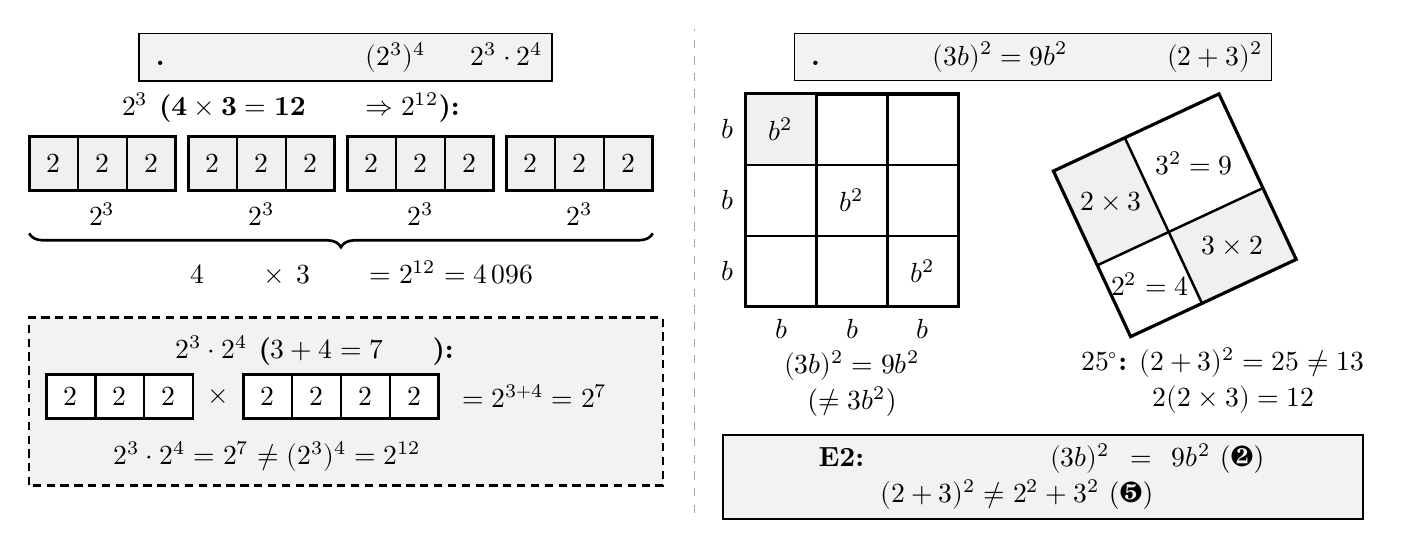
\begin{tikzpicture}[x=1cm, y=1cm, every node/.style={font=\linespread{1.0}\fontsize{10pt}{13pt}\selectfont, text=black}]
  \draw[line width=0.7pt, dashed, gray!70] (8.65, 0.05) -- (8.65, 6.20);
  \node[anchor=north, fill=headgray, draw=black, line width=0.5pt, inner sep=3.2pt] at (4.22, 6.15) {\textbf{ក. ស្ថានីយ៍ ១៖ បន្ទះកត្តា $(2^3)^4$ ធៀប $2^3\cdot 2^4$}};
  \node[anchor=north, fill=headgray, draw=black, line width=0.5pt, inner sep=3.2pt] at (12.95, 6.15) {\textbf{ខ. ស្ថានីយ៍ ២៖ $(3b)^2=9b^2$ និងអន្ទាក់ $(2+3)^2$}};

  \begin{scope}[shift={(0.20, 0.15)}]
    \node[anchor=west] at (0.00, 5.05) {\textbf{៤ បន្ទះនៃ $2^3$ ($\mathbf{4 \times 3 = 12}$ កត្តា $\Rightarrow 2^{12}$):}};
    \foreach \g in {0,1,2,3} {
      \pgfmathsetmacro{\gx}{\g * 2.02}
      \fill[panelgray] (\gx, 4.00) rectangle (\gx+1.86, 4.68);
      \draw[black, line width=1.05pt] (\gx, 4.00) rectangle (\gx+1.86, 4.68);
      \draw[black, line width=0.7pt] (\gx+0.62, 4.00) -- (\gx+0.62, 4.68);
      \draw[black, line width=0.7pt] (\gx+1.24, 4.00) -- (\gx+1.24, 4.68);
      \node at (\gx+0.31, 4.34) {$2$};
      \node at (\gx+0.93, 4.34) {$2$};
      \node at (\gx+1.55, 4.34) {$2$};
      \node[anchor=north] at (\gx+0.93, 3.96) {$2^3$};
    }
    \draw[decorate, decoration={brace, amplitude=5pt, mirror}, black, line width=0.95pt] (0.00, 3.45) -- (7.92, 3.45)
      node[midway, below=6pt] {\textbf{សរុប $4$ ក្រុម $\times$ $3$ កត្តា $= 2^{12} = 4\,096$}};

    \draw[black, densely dashed, line width=0.9pt, fill=headgray] (0.00, 0.25) rectangle (8.05, 2.38);
    \node[anchor=north west] at (0.12, 2.28) {\textbf{ប្រៀបធៀបអន្ទាក់ $2^3 \cdot 2^4$ ($3+4=7$ កត្តា):}};
    \foreach \i in {0,1,2} {
      \fill[white] (0.22+\i*0.62, 1.10) rectangle (0.22+\i*0.62+0.62, 1.66);
      \draw[black, line width=0.9pt] (0.22+\i*0.62, 1.10) rectangle (0.22+\i*0.62+0.62, 1.66);
      \node at (0.22+\i*0.62+0.31, 1.38) {$2$};
    }
    \node at (2.40, 1.38) {\textbf{$\times$}};
    \foreach \j in {0,1,2,3} {
      \fill[white] (2.72+\j*0.62, 1.10) rectangle (2.72+\j*0.62+0.62, 1.66);
      \draw[black, line width=0.9pt] (2.72+\j*0.62, 1.10) rectangle (2.72+\j*0.62+0.62, 1.66);
      \node at (2.72+\j*0.62+0.31, 1.38) {$2$};
    }
    \node[anchor=west] at (5.38, 1.38) {$= 2^{3+4} = 2^7$};
    \node[anchor=west] at (0.14, 0.62) {\textbf{លទ្ធផល៖} $2^3 \cdot 2^4 = 2^7 \neq (2^3)^4 = 2^{12}$};
  \end{scope}

  \begin{scope}[shift={(8.95, 0.15)}]
    \begin{scope}[shift={(0.35, 2.52)}]
      \draw[black, line width=1.15pt] (0,0) rectangle (2.70, 2.70);
      \foreach \x in {0.90, 1.80} {
        \draw[black, line width=0.8pt] (\x, 0) -- (\x, 2.70);
        \draw[black, line width=0.8pt] (0, \x) -- (2.70, \x);
      }
      \fill[panelgray] (0, 1.80) rectangle (0.90, 2.70);
      \draw[black, line width=0.8pt] (0, 1.80) rectangle (0.90, 2.70);
      \node at (0.45, 2.25) {$b^2$};
      \node at (1.35, 1.35) {$b^2$};
      \node at (2.25, 0.45) {$b^2$};
      \node[left=1pt] at (0, 2.25) {$b$};
      \node[left=1pt] at (0, 1.35) {$b$};
      \node[left=1pt] at (0, 0.45) {$b$};
      \node[below=1pt] at (0.45, 0) {$b$};
      \node[below=1pt] at (1.35, 0) {$b$};
      \node[below=1pt] at (2.25, 0) {$b$};
      \node[anchor=north, align=center] at (1.35, -0.44) {\textbf{$(3b)^2 = 9b^2$}\\ ($\neq 3b^2$)};
    \end{scope}

    \begin{scope}[shift={(5.80, 3.68)}, rotate=25]
      \fill[panelgray] (-1.16, -1.16) rectangle (-0.16, 1.16);
      \fill[white] (-1.16, -1.16) rectangle (-0.16, -0.16);
      \fill[panelgray] (-0.16, -1.16) rectangle (1.16, -0.16);
      \draw[black, line width=1.15pt] (-1.16, -1.16) rectangle (1.16, 1.16);
      \draw[black, line width=0.9pt] (-0.16, -1.16) -- (-0.16, 1.16);
      \draw[black, line width=0.9pt] (-1.16, -0.16) -- (1.16, -0.16);
      \node[inner sep=0pt] at (-0.66, -0.66) {$2^2=4$};
      \node at (0.50, 0.50) {$3^2=9$};
      \node at (-0.66, 0.50) {$2\times 3$};
      \node at (0.50, -0.66) {$3\times 2$};
    \end{scope}
    \node[anchor=north, align=center] at (5.80, 2.12) {\textbf{ការ៉េបង្វិល $25^\circ$:} $(2+3)^2=25 \neq 13$\\ \textbf{បាត់ផ្ទៃប្រផេះ} $2(2\times 3)=12$};
    \node[anchor=north west, draw=black, fill=headgray, line width=0.7pt, inner sep=3.2pt, text width=7.90cm] at (0.05, 0.90) {%
      \textbf{សន្និដ្ឋាន \en{E2}:} ស្វ័យគុណចែកចាយលើ\textbf{ផលគុណ} $(3b)^2=9b^2$ (\cnum{2}) តែ\textbf{ហាម}ចែកចាយលើ\textbf{ផលបូក} $(2+3)^2\neq 2^2+3^2$ (\cnum{5})។};
  \end{scope}
\end{tikzpicture}\par
\vspace{2pt}
{\fontsize{10.5pt}{15pt}\selectfont\textbf{រូបទី ១៖} គំរូបន្ទះកត្តា \en{1:1} សម្រាប់ $(2^3)^4 = 2^{12}$ ធៀបនឹង $2^3\cdot 2^4 = 2^7$ និងគំរូក្រឡាការ៉េ $(3b)^2=9b^2$ ទល់នឹងអន្ទាក់ផលបូកបង្វិល $(2+3)^2 \neq 2^2+3^2$ \en{(Gustina et al., 2023; Larbi \& Mavis, 2016; Theba et al., 2024)}។}
\end{tcolorbox}

% --- រូបទី ២ ---
\Needspace{2.2cm}
\begin{tcolorbox}[enhanced, sharp corners, colback=white, colframe=black, boxrule=0.8pt, top=4pt, bottom=4pt, left=5pt, right=5pt, before skip=3pt, after skip=5pt]
\centering
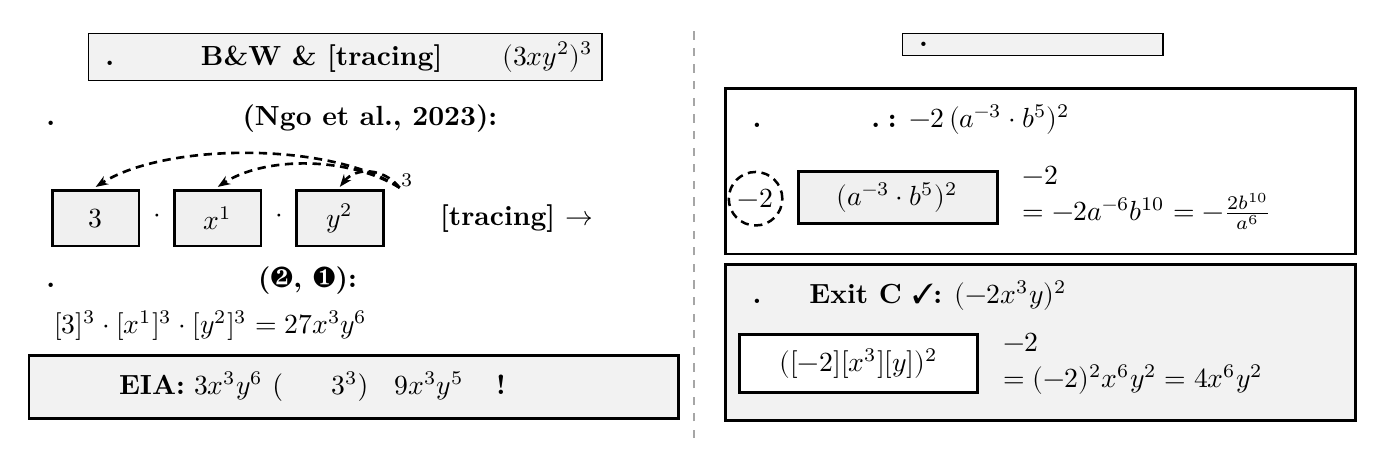
\begin{tikzpicture}[x=1cm, y=1cm, every node/.style={font=\linespread{1.0}\fontsize{10pt}{13pt}\selectfont, text=black}]
  \draw[line width=0.7pt, dashed, gray!70] (8.65, 0.05) -- (8.65, 5.25);
  \node[anchor=north, fill=headgray, draw=black, line width=0.5pt, inner sep=3.2pt] at (4.22, 5.20) {\textbf{ក. វង់ក្រចក \en{B\&W} \& \en{[tracing]} ក្នុង $(3xy^2)^3$}};
  \node[anchor=north, fill=headgray, draw=black, line width=0.5pt, inner sep=3.2pt] at (12.95, 5.20) {\textbf{ខ. វិសាលភាពសញ្ញាដក និងវង់ក្រចក}};

  \begin{scope}[shift={(0.15, 0.15)}]
    \node[anchor=west] at (0.05, 3.96) {\textbf{១. ញែកកត្តាក្នុងវង់ក្រចក (\en{Ngo et al., 2023}):}};
    \draw[black, line width=1.0pt, fill=panelgray] (0.35, 2.34) rectangle (1.45, 3.04);
    \node at (0.90, 2.69) {\textbf{$3$}};
    \node at (1.68, 2.69) {$\cdot$};
    \draw[black, line width=1.0pt, fill=panelgray] (1.90, 2.34) rectangle (3.00, 3.04);
    \node at (2.45, 2.69) {\textbf{$x^1$}};
    \node at (3.23, 2.69) {$\cdot$};
    \draw[black, line width=1.0pt, fill=panelgray] (3.45, 2.34) rectangle (4.55, 3.04);
    \node at (4.00, 2.69) {\textbf{$y^2$}};
    \node[anchor=south west] at (4.66, 2.84) {\textbf{$^3$}};
    \node[anchor=west] at (5.15, 2.69) {\textbf{\en{[tracing]} $\to$ ៣ កត្តា}};

    \draw[black, densely dashed, line width=0.95pt, -{Stealth[length=4.5pt]}] (4.76, 3.08) .. controls (3.90, 3.66) and (1.80, 3.66) .. (0.90, 3.09);
    \draw[black, densely dashed, line width=0.95pt, -{Stealth[length=4.5pt]}] (4.76, 3.08) .. controls (4.10, 3.48) and (3.05, 3.48) .. (2.45, 3.09);
    \draw[black, densely dashed, line width=0.95pt, -{Stealth[length=4.5pt]}] (4.76, 3.08) .. controls (4.55, 3.34) and (4.20, 3.34) .. (4.00, 3.09);

    \node[anchor=west] at (0.05, 1.90) {\textbf{២. ចែកនិទស្សន្តគ្រប់ប្រអប់ (\cnum{2}, \cnum{1}):}};
    \node[anchor=west] at (0.25, 1.33) {$[3]^3 \cdot [x^1]^3 \cdot [y^2]^3 = 27x^3y^6$};
    \draw[black, line width=0.8pt, fill=headgray] (0.05, 0.15) rectangle (8.30, 0.95);
    \node[anchor=west] at (0.15, 0.55) {\textbf{ប្រយ័ត្ន \en{EIA}:} $3x^3y^6$ (ភ្លេច $3^3$) ឬ $9x^3y^5$ \textbf{ខុស!}};
  \end{scope}

  \begin{scope}[shift={(8.95, 0.15)}]
    \draw[black, line width=0.9pt, fill=white] (0.10, 2.24) rectangle (8.10, 4.34);
    \node[anchor=north west] at (0.22, 4.26) {\textbf{ក. ប្រតិបត្តិ ៤.២:} $-2\,(a^{-3}\cdot b^5)^2$};
    \draw[black, line width=0.9pt, densely dashed] (0.48, 2.94) circle (0.34cm);
    \node at (0.48, 2.94) {$-2$};
    \draw[black, line width=1.1pt, fill=panelgray] (1.02, 2.62) rectangle (3.55, 3.28);
    \node at (2.28, 2.95) {$(a^{-3}\cdot b^5)^2$};
    \node[anchor=west, align=left] at (3.75, 2.95) {$-2$ \textbf{នៅក្រៅវង់ក្រចក}\\ $= -2a^{-6}b^{10} = -\tfrac{2b^{10}}{a^6}$};

    \draw[black, line width=1.1pt, fill=headgray] (0.10, 0.12) rectangle (8.10, 2.10);
    \node[anchor=north west] at (0.22, 2.02) {\textbf{ខ. កាត \en{Exit C} \ding{51}:} $(-2x^3y)^2$};
    \draw[black, line width=1.15pt, fill=white] (0.28, 0.48) rectangle (3.30, 1.22);
    \node at (1.79, 0.85) {$([-2][x^3][y])^2$};
    \node[anchor=west, align=left] at (3.50, 0.85) {$-2$ \textbf{នៅក្នុងវង់ក្រចក}\\ $= (-2)^2 x^6 y^2 = 4x^6y^2$};
  \end{scope}
\end{tikzpicture}\par
\vspace{2pt}
{\fontsize{10.5pt}{15pt}\selectfont\textbf{រូបទី ២៖} ការព័ទ្ធវង់ក្រចក ស-ខ្មៅ និងអូសម្រាមដៃ \en{[tracing]} កាត់បន្ថយបន្ទុកគិត ព្រមទាំងបែងចែកវិសាលភាពសញ្ញាដកក្រៅ/ក្នុងវង់ក្រចក \en{(Ngo et al., 2023; Yeo \& Tzeng, 2019; Olson et al., 2011; Booth et al., 2014)}។}
\end{tcolorbox}

% --- រូបទី ៣ ---
\Needspace{2.2cm}
\begin{tcolorbox}[enhanced, sharp corners, colback=white, colframe=black, boxrule=0.8pt, top=4pt, bottom=4pt, left=5pt, right=5pt, before skip=3pt, after skip=5pt]
\centering
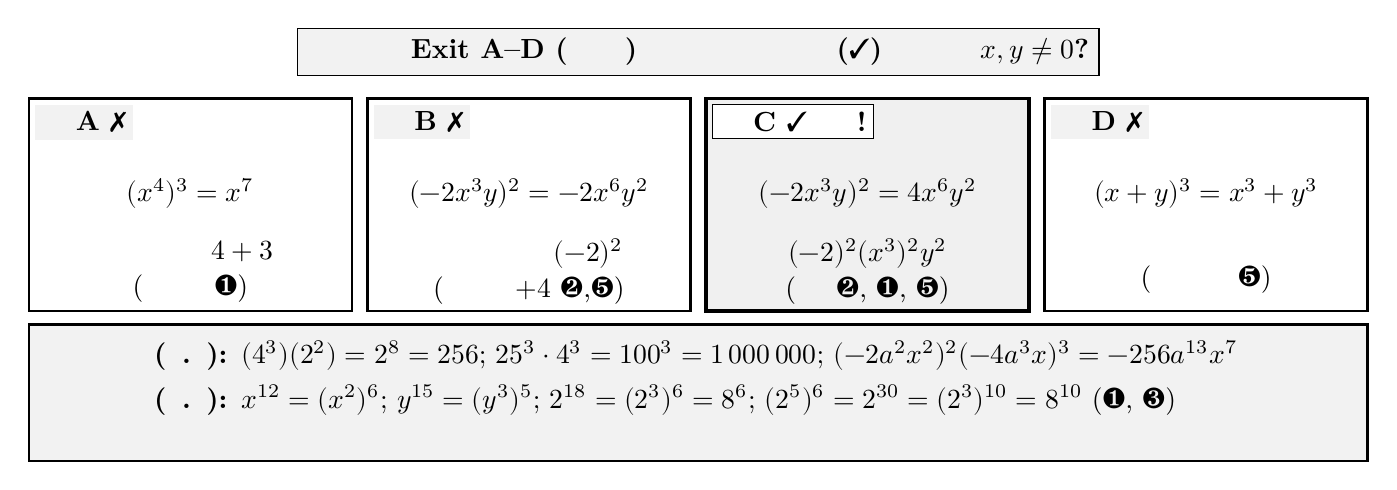
\begin{tikzpicture}[x=1cm, y=1cm, every node/.style={font=\linespread{1.0}\fontsize{10pt}{13pt}\selectfont, text=black}]
  \node[anchor=north, fill=headgray, draw=black, line width=0.6pt, inner sep=3.5pt] at (8.55, 5.25) {\textbf{កាតវិនិច្ឆ័យ \en{Exit A--D} (ទំព័រ ៥)៖ តើសមភាពមួយណាត្រឹមត្រូវ (\ding{51}) ចំពោះគ្រប់ $x, y \neq 0$?}};

  \draw[black, line width=0.95pt] (0.05, 1.65) rectangle (4.15, 4.35);
  \node[anchor=north west, fill=headgray, inner sep=2.5pt] at (0.12, 4.28) {\textbf{កាត \en{A} \ding{55}}};
  \node[align=center] at (2.10, 3.15) {$(x^4)^3 = x^7$};
  \node[align=center] at (2.10, 2.15) {អន្ទាក់៖ បូក $4+3$\\ (\textit{ត្រូវគុណ} \cnum{1})};

  \draw[black, line width=0.95pt] (4.35, 1.65) rectangle (8.45, 4.35);
  \node[anchor=north west, fill=headgray, inner sep=2.5pt] at (4.42, 4.28) {\textbf{កាត \en{B} \ding{55}}};
  \node[align=center] at (6.40, 3.15) {$(-2x^3y)^2 = -2x^6y^2$};
  \node[align=center] at (6.40, 2.15) {អន្ទាក់៖ ភ្លេច $(-2)^2$\\ (\textit{ត្រូវបាន $+4$} \cnum{2},\cnum{5})};

  \draw[black, line width=1.35pt, fill=panelgray] (8.65, 1.65) rectangle (12.75, 4.35);
  \node[anchor=north west, fill=white, draw=black, line width=0.5pt, inner sep=2.5pt] at (8.72, 4.28) {\textbf{កាត \en{C} \ding{51} ត្រូវ!}};
  \node[align=center] at (10.70, 3.15) {\textbf{$(-2x^3y)^2 = 4x^6y^2$}};
  \node[align=center] at (10.70, 2.15) {$(-2)^2(x^3)^2y^2$\\ (\textit{ប្រើ} \cnum{2}, \cnum{1}, \cnum{5})};

  \draw[black, line width=0.95pt] (12.95, 1.65) rectangle (17.05, 4.35);
  \node[anchor=north west, fill=headgray, inner sep=2.5pt] at (13.02, 4.28) {\textbf{កាត \en{D} \ding{55}}};
  \node[align=center] at (15.00, 3.15) {$(x+y)^3 = x^3 + y^3$};
  \node[align=center] at (15.00, 2.15) {អន្ទាក់៖ លីនេអ៊ែរ\\ (\textit{ហាមលើផលបូក} \cnum{5})};

  \draw[black, line width=0.85pt, fill=headgray] (0.05, -0.25) rectangle (17.05, 1.48);
  \node[anchor=north west, text width=16.65cm] at (0.18, 1.40) {\textbf{ផ្ទះ ផ្នែក ក (ទំ.២៥):} $(4^3)(2^2)=2^8=256$; $25^3\cdot 4^3=100^3=1\,000\,000$; $(-2a^2x^2)^2(-4a^3x)^3=-256a^{13}x^7$\\[3pt]
  \textbf{ផ្ទះ ផ្នែក ខ (ទំ.២៦):} $x^{12}=(x^2)^6$; $y^{15}=(y^3)^5$; $2^{18}=(2^3)^6=8^6$; $(2^5)^6=2^{30}=(2^3)^{10}=8^{10}$ (\cnum{1}, \cnum{3})};
\end{tikzpicture}\par
\vspace{2pt}
{\fontsize{10.5pt}{15pt}\selectfont\textbf{រូបទី ៣៖} ផែនទីវិនិច្ឆ័យកាត \en{Exit A--D} (ទំព័រ ៥) ចាប់កំហុសទាំង ៤ និងការផ្សារភ្ជាប់ទៅកិច្ចការផ្ទះទំព័រ ២៥--២៦ \en{(Klingbeil et al., 2024; Şenay, 2024; Ulusoy, 2019)}។}
\end{tcolorbox}

% ============================================================================
% ផ្នែកទី ៤៖ សេណារីយ៉ូពាក្យពេចន៍គ្រូបង្រៀនផ្ទាល់ និងការគ្រប់គ្រងក្ដារខៀន
% ============================================================================
\secbanner{ផ្នែកទី ៤៖ សេណារីយ៉ូពាក្យពេចន៍គ្រូបង្រៀនផ្ទាល់ និងការគ្រប់គ្រងក្ដារខៀន}{Section 4: Verbatim Teacher Scripts (00--50 min), Pause-Ask/Review Gates \& 3-Zone Blackboard Plan}

សេណារីយ៉ូបង្រៀនផ្ទាល់ខាងក្រោមត្រូវបានបំបែកតាមវគ្គនីមួយៗ ដើម្បីឱ្យគ្រូអានបានស្រួលនៅលើអេក្រង់ទូរស័ព្ទ ដោយរក្សាភាពស៊ីចង្វាក់ ១០០\% ជាមួយ \en{LS\_Plan\_EXP412} និង \en{Teaching\_Scenario\_EXP412}។

\Needspace{2.0cm}
\begin{phasebox}{ជំហាន ១ \enbf{\&} ២ក\enbf{--}ខ៖ រដ្ឋបាល កំណែលំហាត់ទំ\enbf{.}១៦ និងរំលឹក}{00--08 min}{8 នាទី}
\textbf{គោលបំណង}៖ រៀបចំក្រុម ៣ នាក់, ផ្ទៀងប្រតិបត្តិទំ.១៦ ទប់អន្ទាក់ $a^0=1$ និង $a^{-n}=\frac{1}{a^n}$, រួចរំលឹក $a^m\cdot a^n=a^{m+n}$ \en{(Ulusoy, 2019; Turan \& Matteson, 2021)}។
\end{phasebox}
\begin{scriptbox}
  \textbf{នាទី \en{00--02} (រដ្ឋបាល) — }\teachersays{សួស្ដីប្អូនៗ! ថ្ងៃនេះក្រុម ៣ នាក់របស់យើងមានតួនាទី ៣៖ តួនាទី ១ (អ្នកគូសវង់ក្រចក \en{B\&W} និងអូស \en{[tracing]}), តួនាទី ២ (អ្នកភ្ជាប់ហេតុផល \cnum{1}--\cnum{5} និងគណនា) និងតួនាទី ៣ (អ្នកត្រួតពិនិត្យសញ្ញាដក-លក្ខខណ្ឌ)។ សូមរៀបកន្ត្រៃ និងបន្ទាត់ \en{cm} លើតុ ហើយដាក់ក្រដាសទំព័រ ១ ផ្កាប់ចុះក្រោមសិន — កុំទាន់កាត់មុនបញ្ជាគ្រូ!}\par\vspace{3pt}
  \textbf{នាទី \en{02--05} (កំណែទំ.១៦ $\le 3'$) — }\teachersays{ផ្ទៀងលំហាត់ \textbf{ប្រតិបត្តិ ទំ.១៦ (ក--ឃ)}៖ \textbf{ក.} $\frac{x^9}{x^4} = x^{9-4} = x^5$ ($x \neq 0$)។ \textbf{ខ.} $\frac{(3/2)^2}{(3/2)^4} = (3/2)^{2-4} = (3/2)^{-2} = \frac{1}{(3/2)^2} = \frac{4}{9}$ (កុំដាក់សញ្ញាដកពីមុខ $\frac{4}{9}$ ណា ព្រោះនិទស្សន្តដកប្រែជាចម្រាស!)។ \textbf{គ.} $\frac{y^9}{y^9} = y^0 = 1$ ($y \neq 0$)។ \textbf{ឃ.} $\left(\frac{3yx^9}{-15y^5x^4}\right)^0 = 1$ ($x, y \neq 0$) — សម្រាប់ \textbf{ឃ.} តើត្រូវចំណាយពេលសម្រួលខាងក្នុងទេ?}\par\vspace{2pt}
  \textbf{$\circ$ សិស្ស៖} \textit{«ទេលោកគ្រូ! ព្រោះវង់ក្រចកទាំងមូលលើកស្វ័យគុណសូន្យស្មើ ១ ភ្លាម!»}\par\vspace{3pt}
  \textbf{នាទី \en{05--08} (រំលឹក ៣') — }\teachersays{រំលឹករហ័ស៖ \textbf{១)} $a^n = a\cdot a\cdots a$ ($n$ កត្តា) និង $a^{-n} = \frac{1}{a^n}$ ($a \neq 0$)។ \textbf{២)} ពេលគុណស្វ័យគុណគោលដូចគ្នា $a^m \cdot a^n$ តើនិទស្សន្តធ្វើអ្វី?}\par\vspace{2pt}
  \textbf{$\circ$ សិស្ស៖} \textit{«បូកនិទស្សន្ត $a^{m+n}$ ដូចជា $2^3\cdot 2^4 = 2^{3+4} = 2^7$!»} (គ្រូសរសេរ $2^3\cdot 2^4=2^7$ ទុកលើក្ដារខៀនឆ្វេង)។
\end{scriptbox}

\Needspace{2.0cm}
\begin{phasebox}{ជំហាន ២គ \enbf{(E1 - Engage)}៖ បេសកកម្មអង្គចងចាំកុំព្យូទ័រ និងការ៉ូការ៉េ}{08--11 min}{3 នាទី}
\textbf{គោលបំណង}៖ បង្កើតជម្លោះគំនិតរវាងការទស្សន៍ទាយរបស់សុខនិងបូណាលើ $(2^3)^4$ និង $(3b)^2$ \en{(Ellis et al., 2013; Gustina et al., 2023)}។
\end{phasebox}
\begin{scriptbox}
  \textbf{នាទី \en{08--11} — }\teachersays{មើលបេសកកម្ម ២ លើក្ដារខៀន៖ \textbf{ស្ថានភាពទី ១ (៤.១)៖} អង្គចងចាំកុំព្យូទ័រពង្រីក ៤ តំណាក់កាល ដែលក្នុង ១ កញ្ចប់មាន $2^3$ បៃ សរសេរជា $(2^3)^4$ បៃ។ \textbf{សុខ} ថា $(2^3)^4 = 2^{3+4} = 2^7 = 128$ បៃ; រីឯ \textbf{បូណា} ថា $(2^3)^4 = 2^{3\times 4} = 2^{12} = 4\,096$ បៃ។ \textbf{ស្ថានភាពទី ២ (៤.២)៖} ការ៉េធំជ្រុង $(3b)\unit{cm}$ ផ្សំពីការ៉ូតូចជ្រុង $b\unit{cm}$។ \textbf{សុខ} ថា $(3b)^2 = 3b^2$ (៣ ការ៉ូ); រីឯ \textbf{បូណា} ថា $(3b)^2 = 9b^2$ (៩ ការ៉ូ)។ តើក្រុមប្អូនកាន់ខាង \textbf{សុខ} ឬ \textbf{បូណា}?}\par\vspace{2pt}
  \textbf{$\circ$ សកម្មភាពសិស្ស៖} ក្រុមលើកដៃបោះឆ្នោតជ្រើសទស្សន៍ទាយ។ គ្រូកត់ចំនួនទុកលើក្ដារខៀន \textbf{ដោយមិនទាន់បញ្ជាក់ចម្លើយត្រូវ} រួចបើកការពិសោធន៍ \en{1:1}។
\end{scriptbox}

\Needspace{2.0cm}
\begin{phasebox}{ជំហាន ៣ក \enbf{(E2 - Explore} ស្ថានីយ៍ ១\enbf{)}៖ បន្ទះកត្តា ១\enbf{:}១ សម្រាប់ $(2^3)^4$}{11--16 min}{5 នាទី}
\textbf{គោលបំណង}៖ សិស្សរកឃើញថា $(2^3)^4 = 2^{3\times 4} = 2^{12}$ តាមរយៈ ៤ បន្ទះនៃ $2^3$ និងញែកចេញពី $2^3\cdot 2^4 = 2^7$ \en{(Gustina et al., 2023; Ulusoy, 2019)}។
\end{phasebox}
\begin{scriptbox}
  \textbf{នាទី \en{11--16} (ទំព័រ ១ ស្ថានីយ៍ ១) — }\teachersays{ត្រឡប់ទំព័រ ១ ឡើង! មុនកាត់ យកបន្ទាត់វាស់ \textbf{ក្រិត $5.00\unit{cm}$} ខាងលើឱ្យច្បាស់ថាត្រូវខ្នាត \en{1:1}។ កាត់ \textbf{៤ បន្ទះនៃ $2^3$} (បន្ទះនីមួយៗប្រវែង $3.0\unit{cm}$ មាន ៣ ក្រឡា $2\cdot 2\cdot 2$)។ មុនតម្រៀបចូលប្រអប់គោលដៅ $12.0\unit{cm}$ សូមគូសប្រអប់ \textbf{ទស្សន៍ទាយ (\en{P})} ជាមុន! ឥឡូវតម្រៀបបន្ទះទាំង ៤ តគ្នាក្នុងប្រអប់ \textbf{សង្កេត (\en{O})} ហើយយកម្រាមដៃ \textbf{\en{[tracing]}} រាប់កត្តា $2$ ពីឆ្វេងទៅស្ដាំ!}\par\vspace{2pt}
  \textbf{$\circ$ សិស្ស៖} \textit{«មាន ១២ កត្តាគុណគ្នា! $(2^3)^4 = 2^{3+3+3+3} = 2^{3\times 4} = 2^{12}$!»}\par\vspace{3pt}
  \teachersays{ល្អណាស់! ចុះក្នុង \textbf{ឧទាហរណ៍ ៤.១ ខ (ទំ.១៧)} តើ $(5^6)^4$ បានប៉ុន្មាន? ហើយតើ $(2^3)^4$ ស្មើ $(2^4)^3$ ទេ? ហេតុអ្វី $2^3\cdot 2^4 = 2^7$ ខុសពី $(2^3)^4 = 2^{12}$?}\par\vspace{2pt}
  \textbf{$\circ$ សិស្ស៖} \textit{«$(5^6)^4 = 5^{6\times 4} = 5^{24}$; $(2^3)^4 = (2^4)^3 = 2^{12}$; ឯ $2^3\cdot 2^4 = 2^{3+4} = 2^7$ ជាគោលដូចគ្នាបូកនិទស្សន្ត មិនមែន ៤ ក្រុមនៃ ៣ ទេ!»}
\end{scriptbox}

\Needspace{2.0cm}
\begin{phasebox}{ជំហាន ៣ក \enbf{(E2 - Explore} ស្ថានីយ៍ ២\enbf{)}៖ ក្រឡា \enbf{6x6 cm} និងការ៉េបង្វិល $25^\circ$}{16--22 min}{6 នាទី}
\textbf{គោលបំណង}៖ សិស្សរកឃើញ $a^n\cdot b^n = (ab)^n$, $(3b)^2 = 9b^2$ និងទាត់ចោល $(2+3)^2 = 2^2+3^2$ \en{(Larbi \& Mavis, 2016; Theba et al., 2024)}។
\end{phasebox}
\begin{scriptbox}
  \textbf{នាទី \en{16--22} (ទំព័រ ១ ស្ថានីយ៍ ២) — }\teachersays{ចូលស្ថានីយ៍ទី ២! មើលផ្នែក \en{A} (\textbf{ទំ.១៧ ក, ខ, គ})៖ \textbf{ក.} $2^3\times 5^3$ ផ្គុំគូ $(2\times 5)$ បានប៉ុន្មានក្រុម? \textbf{ខ.} ចុះ $2^2\times 5^2\times 7^2$? \textbf{គ.} ចុះ $a^n\cdot b^n$?}\par\vspace{2pt}
  \textbf{$\circ$ សិស្ស៖} \textit{«ក. $(2\times 5)^3 = 10^3 = 1\,000$; ខ. $(2\times 5\times 7)^2 = 70^2 = 4\,900$; គ. $a^n\cdot b^n = (ab)^n$!»}\par\vspace{3pt}
  \teachersays{ឥឡូវមើលផ្នែក \en{B}៖ \textbf{ក្រឡាការ៉េ $6.0\unit{cm}\times 6.0\unit{cm}$} (ដែល $b=2.0\unit{cm}$, ជ្រុង $3b=6.0\unit{cm}$) ផ្ទុកការ៉ូតូច $b^2$ ប៉ុន្មានផ្ទាំង? ហើយមើល \textbf{ការ៉េបង្វិល $25^\circ$} ជ្រុង $(2+3)$ — តើ $(2+3)^2$ ស្មើ $2^2+3^2$ ដែរឬទេ?}\par\vspace{2pt}
  \textbf{$\circ$ សិស្ស៖} \textit{«ការ៉េ $3b\times 3b$ មាន ៩ ការ៉ូ $b^2 \Rightarrow (3b)^2 = 9b^2 \neq 3b^2$! រីឯការ៉េបង្វិល $(2+3)^2 = 25 \neq 2^2+3^2 = 13$ ព្រោះបាត់ចតុកោណកែងប្រផេះ ២ ផ្ទាំង $2\times(2\times 3)=12$!»}
\end{scriptbox}

\Needspace{2.0cm}
\begin{phasebox}{ជំហាន ៣ខ \enbf{(E3 - Explain)}៖ បង្គុំទ្រឹស្ដីបទ ៤\enbf{.}១\enbf{--}៤\enbf{.}២ និង \enbf{Warrant Bank} \cnum{1}\enbf{--}\cnum{5}}{22--28 min}{6 នាទី}
\textbf{គោលបំណង}៖ សិស្សបង្គុំប្រអប់ «ជាទូទៅ» (រួមទាំង $a\neq 0, b\neq 0$), ឆ្លើយសំណួរ \en{Beeth} និងប្រើផ្ទាំង \cnum{1}--\cnum{5} \en{(Runisah et al., 2017; Vest et al., 2022)}។
\end{phasebox}
\begin{scriptbox}
  \textbf{នាទី \en{22--28} (ទំព័រ ៤) — }\teachersays{សូមសិស្សជួយគ្រូបំពេញ \textbf{ប្រអប់ «ជាទូទៅ» ៤.១ និង ៤.២ (ទំ.១៧)}៖ ចំពោះ $a, b$ ជាចំនួនសនិទាន និង $m, n$ ជាចំនួនគត់រ៉ឺឡាទីបខុសពីសូន្យ គេបាន $(a^m)^n = (a^n)^m = a^{m\cdot n}$ និង $(a\cdot b)^n = a^n\cdot b^n$។ ប្រយ័ត្ន! ពេល $m<0$ ឬ $n<0$ តើត្រូវបន្ថែមលក្ខខណ្ឌអ្វី?}\par\vspace{2pt}
  \textbf{$\circ$ សិស្ស៖} \textit{«ត្រូវ $a \neq 0$ និង $b \neq 0$ ដើម្បីកុំឱ្យភាគបែងស្មើសូន្យ!»}\par\vspace{3pt}
  \teachersays{ឆ្លើយ \textbf{សំណួរមេតាកូញីទីវ \en{Beeth} ទាំង ៣}៖ \textbf{១) ភាពងាយយល់៖} ហេតុអ្វី $(a^m)^n$ គុណនិទស្សន្ត ឯ $a^m\cdot a^n$ បូកនិទស្សន្ត? \textbf{២) ភាពសមហេតុផល៖} ហេតុអ្វី $(3b)^2=9b^2$ ពិត តែ $(2+3)^2 \neq 2^2+3^2$? \textbf{៣) ភាពប្រើបានទូលំទូលាយ៖} បើជួប $25^3\cdot 4^3$ តើធ្វើដូចម្ដេចលឿនបំផុត?}\par\vspace{2pt}
  \textbf{$\circ$ សិស្ស៖} \textit{«ប្រើទិសច្រាស \cnum{3}៖ $25^3\cdot 4^3 = (25\times 4)^3 = 100^3 = 1\,000\,000$!»} (គ្រូបិទ \textbf{ផ្ទាំងធនាគារហេតុផល \cnum{1}--\cnum{5} ទំព័រ ៤} លើក្ដារខៀនកណ្ដាល)។
\end{scriptbox}

\Needspace{2.0cm}
\begin{phasebox}{ជំហាន ៤ក \enbf{(E4 - Elaborate)}៖ កាតស៊ើបអង្កេត \enbf{B\&W} លំហាត់គំរូទំ\enbf{.}១៧\enbf{--}១៨}{28--38 min}{10 នាទី}
\textbf{គោលបំណង}៖ ហ្វឹកហាត់កាត ៣ ជំហាន \en{([tracing]} + វង់ក្រចក \en{B\&W} + \cnum{1}--\cnum{5}) និង \en{EIA Looking-Back} \en{(Özcan, 2024; Yeo \& Tzeng, 2019; Ngo et al., 2023)}។
\end{phasebox}
\begin{scriptbox}
  \textbf{នាទី \en{28--38} (ទំព័រ ២) — }\teachersays{ចែកកាត \en{E4} (ទំព័រ ២)! ធ្វើតាម ៣ ជំហាន៖ ១) ព័ទ្ធវង់ក្រចក-អូស \en{[tracing]}, ២) ចុះលេខ \cnum{1}--\cnum{5} គណនា, ៣) \en{EIA Looking-Back}។ មើល \textbf{គំរូ ៤.១ (ទំ.១៧)}៖ \textbf{ក.} $(10^2)^3 = 10^{2\times 3} = 10^6 = 1\,000\,000$ (\cnum{1}); \textbf{ខ.} $(a^{-2})^k(a^k)^5 = a^{-2k}\cdot a^{5k} = a^{3k}$ (\cnum{1}, \cnum{4}, $a\neq 0$)។ មើល \textbf{គំរូ ៤.២ (ទំ.១៨)}៖ \textbf{ក.} $(3xy^2)^3$ — សូមព័ទ្ធប្រអប់ \textbf{$([3]\cdot[x^1]\cdot[y^2])^3$} រួចអូស \en{[tracing]} ចង្អុលនិទស្សន្ត $3$ ចូលគ្រប់ប្រអប់ទាំង ៣ បាន $3^3\cdot x^3\cdot(y^2)^3 = 27x^3y^6$ (\cnum{2}, \cnum{1})! \textbf{ខ.} $(b^3)(b^{2k-1})^3 = b^3\cdot b^{3(2k-1)} = b^{3+6k-3} = b^{6k}$ (\cnum{1}, \cnum{4}, $b\neq 0$)។}\par\vspace{3pt}
  \teachersays{\textbf{សំណួរ \en{EIA Looking-Back}:} ១) ហេតុអ្វី $(3xy^2)^3 = 3x^3y^6$ ឬ $9x^3y^5$ ខុស? ២) ហេតុអ្វី $b^{3(2k-1)} \neq b^{6k-1}$?}\par\vspace{2pt}
  \textbf{$\circ$ សិស្ស៖} \textit{«១) ទីមួយភ្លេច $3^3=27$ (\cnum{2}) ទីពីរគុណ-បូកច្រឡំ; ២) ត្រូវគុណ $3$ ចូល $-1$ ផងដែរជា $6k-3$!»}
\end{scriptbox}

\Needspace{2.0cm}
\begin{phasebox}{ជំហាន ៤ខ \enbf{(E5 - Evaluate)}៖ \enbf{Relay} ៣ តួនាទី \enbf{(Pause-Ask/Review)} និងបិទ \enbf{E1}}{38--45.5 min}{7.5 នាទី}
\textbf{គោលបំណង}៖ ផ្ទេរជំនាញលើប្រតិបត្តិទំ.១៧--១៨ ដោយសហការ ៣ តួនាទី និងផ្ទៀងវិសាលភាព $-2(a^{-3}b^5)^2$ \en{(Olson et al., 2011; Vest et al., 2022)}។
\end{phasebox}
\begin{scriptbox}
  \textbf{នាទី \en{38--44} (ទំព័រ ៣) — }\teachersays{ចែកសន្លឹក \textbf{Relay ៣ តួនាទី (ទំព័រ ៣)}! \textbf{បេសកកម្ម A (៤.១ ទំ.១៧)}៖ ក. $(a^3)^{-2}$, ខ. $a\cdot(a^4)^5\cdot a^{-6}$ និង \textbf{បេសកកម្ម B (៤.២ ទំ.១៨)}៖ ក. $-2(a^{-3}\cdot b^5)^2$, ខ. $a\cdot(a^4)\cdot a^{-6}$។ \textbf{តួនាទី ១ (\en{Pause-Ask!})៖} ព័ទ្ធរង្វង់ $-2$ ក្រៅវង់ក្រចក ដាក់ $a^1$ អូស \en{[tracing]} ហើយសួរដៃគូ៖ \textit{«តើ $-2$ នៅក្នុងឬក្រៅស្វ័យគុណ $2$? ចុះ $a\cdot(a^4)\cdot a^{-6}$ ទំ.១៨ មានស្វ័យគុណ $5$ ខាងក្រៅទេ?»}}\par\vspace{2pt}
  \textbf{$\circ$ សិស្ស៖} \textit{«$-2$ នៅក្រៅ មិនលើកស្វ័យគុណ $2$ ទេ! ឯទំ.១៨ គ្មាននិទស្សន្ត $5$ ខាងក្រៅទេ!»}\par\vspace{3pt}
  \teachersays{\textbf{តួនាទី ២} គណនាភ្ជាប់ \cnum{1}--\cnum{5}៖ A.ក $=a^{-6}=\frac{1}{a^6}$, A.ខ $=a^{1+20-6}=a^{15}$; B.ក $=-2a^{-6}b^{10}=-\frac{2b^{10}}{a^6}$, B.ខ $=a^{1+4-6}=a^{-1}=\frac{1}{a}$ ($a\neq 0$)។ \textbf{តួនាទី ៣ (\en{Pause-Review!})៖} ត្រួតពិនិត្យសញ្ញាដកមុខ $-\frac{2b^{10}}{a^6}$ លក្ខខណ្ឌ $a\neq 0$ និងប្រៀបធៀប $a^{15}$ (ទំ.១៧) ទល់នឹង $\frac{1}{a}$ (ទំ.១៨)!}\par\vspace{3pt}
  \textbf{នាទី \en{44--45.5} (បិទ \en{E1}) — }\teachersays{ត្រឡប់ទៅការទស្សន៍ទាយដើមម៉ោង! តើសុខ ឬបូណាត្រូវ?}\par\vspace{2pt}
  \textbf{$\circ$ សិស្ស៖} \textit{«បូណាត្រូវទាំងពីរ! $(2^3)^4 = 2^{12} = 4\,096$ (\cnum{1}) និង $(3b)^2 = 9b^2$ (\cnum{2})!»}
\end{scriptbox}

\Needspace{2.0cm}
\begin{phasebox}{ជំហាន ៤ខ \enbf{(E5 Exit)} និង ៥៖ កាត \enbf{A--D} ៩០ វិនាទី និងកិច្ចការផ្ទះ}{45.5--50 min}{4.5 នាទី}
\textbf{គោលបំណង}៖ វាយតម្លៃកំហុសទាំង ៤ ក្នុង ៩០ វិនាទី (\en{Klingbeil et al., 2024}) និងចែកកិច្ចការផ្ទះទំ.២៥--២៦ (\en{Booth et al., 2014})។
\end{phasebox}
\begin{scriptbox}
  \textbf{នាទី \en{45.5--48} (ទំព័រ ៥) — }\teachersays{មើលកាត \en{Exit A--D} ហើយលើកកាតឆ្លើយព្រមគ្នាក្នុង ៣ វិនាទី៖ \textit{«តើសមភាពមួយណាត្រឹមត្រូវ (\ding{51}) ចំពោះគ្រប់ $x, y \neq 0$?»} \textbf{A:} $(x^4)^3=x^7$; \textbf{B:} $(-2x^3y)^2=-2x^6y^2$; \textbf{C:} $(-2x^3y)^2=4x^6y^2$; \textbf{D:} $(x+y)^3=x^3+y^3$។ ១, ២, ៣ — លើក! \textbf{C} ត្រឹមត្រូវ! បើអ្នកណាលើក A, B ឬ D គ្រូកែកំហុសភ្លាមតាមសោទំព័រ ៥ រួចប្រមូលចម្លើយ។}\par\vspace{3pt}
  \textbf{នាទី \en{48--50} (កិច្ចការផ្ទះ ទំព័រ ៦) — }\teachersays{ចែកប័ណ្ណកិច្ចការផ្ទះ (ទំព័រ ៦, ទំ.២៥--២៦)៖ \textbf{ផ្នែក ក៖} ១) គណនា $(4^3)(2^2)$ ដោយប្ដូរ $4=2^2$ (ទំ.២៥ \#២ក) និង $25^3\cdot 4^3$ ដោយ \cnum{3}; ២) សម្រួល $(-2a^2x^2)^2(-4a^3x)^3$ (ត្រៀម \#៧ង)។ \textbf{ផ្នែក ខ៖} ១) សរសេរ $x^{12}$ ជាស្វ័យគុណនៃ $x^2$ និង $y^{15}$ ជាស្វ័យគុណនៃ $y^3$ (ទំ.២៦ \#៨ក,ខ); ២) សរសេរ $2^{18}$ និង $(2^5)^6$ ជាស្វ័យគុណនៃ $8$ (ទំ.២៦ \#៨គ)។ អានមុន \textbf{២.៤.៣ ស្វ័យគុណនៃផលចែក} នៅទំព័រ ១៨!}
\end{scriptbox}

\subsec{៤\enbf{.}១ ប្លង់រៀបចំក្ដារខៀន ៣ ផ្នែក \enbf{(Blackboard Layout)}}

{\linespread{1.0}\fontsize{10.0pt}{14.5pt}\selectfont
\setlength{\LTpre}{4pt}\setlength{\LTpost}{4pt}
\begin{longtable}{|L{5.50cm}|L{5.90cm}|L{5.80cm}|}
\hline
\rowcolor{headgray}
\multicolumn{1}{|L{5.50cm}|}{\tblhead{ផ្នែកឆ្វេង៖ រំលឹក\enbf{, E1 \& E2}}} &
\multicolumn{1}{L{5.90cm}|}{\tblhead{ផ្នែកកណ្ដាល៖ ទ្រឹស្ដី ៤\enbf{.}១\enbf{--}៤\enbf{.}២ \enbf{\&} \cnum{1}\enbf{--}\cnum{5}}} &
\multicolumn{1}{L{5.80cm}|}{\tblhead{ផ្នែកស្ដាំ៖ \enbf{E4, E5 \&} កិច្ចការផ្ទះ}} \\
\hline
\endfirsthead
\hline
\rowcolor{headgray}
\multicolumn{1}{|L{5.50cm}|}{\tblhead{ផ្នែកឆ្វេង៖ រំលឹក\enbf{, E1 \& E2}}} &
\multicolumn{1}{L{5.90cm}|}{\tblhead{ផ្នែកកណ្ដាល៖ ទ្រឹស្ដី ៤\enbf{.}១\enbf{--}៤\enbf{.}២ \enbf{\&} \cnum{1}\enbf{--}\cnum{5}}} &
\multicolumn{1}{L{5.80cm}|}{\tblhead{ផ្នែកស្ដាំ៖ \enbf{E4, E5 \&} កិច្ចការផ្ទះ}} \\
\hline
\endhead
\hline
\endfoot
\hline
\endlastfoot
\ditem កែទំ.១៦៖ $x^5,\; \frac{4}{9},\; 1,\; 1$ \newline
\ditem រំលឹក៖ $2^3\cdot 2^4 = 2^7$ &
\ditem \textbf{៤.១:} $(a^m)^n=(a^n)^m=a^{m\cdot n}$ \newline
\ditem \textbf{៤.២:} $(a\cdot b)^n = a^n\cdot b^n$ &
\ditem \textbf{E4:} $(10^2)^3=10^6$; $a^{3k}$ \newline
\ditem $([3][x^1][y^2])^3 = 27x^3y^6$; $b^{6k}$ \\[3pt]
\ditem \textbf{E1}: $(2^3)^4$ (សុខ vs បូណា) \newline
\ditem \textbf{E2 (ស.១)}: $(2^3)^4 = 2^{12} \neq 2^7$ &
\ditem លក្ខខណ្ឌ $a\neq 0, b\neq 0$ ($m,n<0$) \newline
\ditem ផ្ទាំង \textbf{ធនាគារ \cnum{1}--\cnum{5}} (ទំ. ៤) &
\ditem \textbf{E5 (ទំ.៣)}: $\frac{1}{a^6}, a^{15}, -\frac{2b^{10}}{a^6}, \frac{1}{a}$ \newline
\ditem \textbf{Exit}: កាត \textbf{C \ding{51}} ($4x^6y^2$) \\[3pt]
\ditem \textbf{E2 (ស.២)}: $(3b)^2=9b^2$ \newline
\ditem $(2+3)^2 = 25 \neq 2^2+3^2$ &
\ditem ច្រាស៖ $25^3\cdot 4^3 = 100^3$ \newline
\ditem ហាម៖ $(a+b)^n \neq a^n+b^n$ &
\ditem \textbf{បិទ E1}: បូណាត្រូវ ($2^{12}, 9b^2$) \newline
\ditem \textbf{ផ្ទះ} ទំ.២៥--២៦ (\en{\#2}ក, \en{\#7}ង, \en{\#8}) \\
\hline
\end{longtable}
}

% ============================================================================
% ផ្នែកទី ៥៖ មគ្គុទ្ទេសក៍វិនិច្ឆ័យកំហុស និងការជួសជុលបន្ទាន់ (Troubleshooting Guide)
% ============================================================================
\secbanner{ផ្នែកទី ៥៖ មគ្គុទ្ទេសក៍វិនិច្ឆ័យកំហុស និងការជួសជុលបន្ទាន់}{Section 5: Step-by-Step Misconception Remediation Guide \& Book p. 18 Print Note}

\subsec{៥\enbf{.}១ វិធានការកែតម្រូវរហ័ស ៣០ វិនាទីតាមករណីនីមួយៗ}

\begin{enumerate}[leftmargin=0.65cm]
  \item \textbf{អន្ទាក់បូកនិទស្សន្ត $(a^m)^n = a^{m+n}$ (\en{Ulusoy, 2019; Şenay, 2024})៖} នៅពេលឃើញសិស្សសរសេរ $(2^3)^4=2^7$ ឬជ្រើសកាត \en{A} $(x^4)^3=x^7$ គ្រូមិនគួរប្រាប់ត្រង់ៗថា \textit{«ខុស ត្រូវគុណវិញ»} ឡើយ។ ឱ្យសិស្សប៉ះបន្ទះកាត់ទំ.១ ឡើងវិញហើយសួរ៖ \textit{«ប្រសិនបើមានបន្ទះ $2^3$ ចំនួន ៤ បន្ទះតម្រៀបគ្នា តើមានលេខ $2$ គុណគ្នា $3+4=7$ តួ ឬ $4$ ក្រុមនៃ $3$ តួ?»} រួចប្រៀបធៀបទល់នឹង $2^3\cdot 2^4 = 2^7$។
  \item \textbf{អារម្មណ៍បំភាន់លីនេអ៊ែរ $(a+b)^n = a^n+b^n$ (\en{Theba et al., 2024; Larbi \& Mavis, 2016})៖} ពេលសិស្សជឿថាកាត \en{D} $(x+y)^3=x^3+y^3$ ឬ $(2+3)^2=2^2+3^2$ ត្រឹមត្រូវ គ្រូដាក់ក្រឡា \en{1:1} ការ៉េបង្វិល $25^\circ$ (ទំ.១) នៅមុខសិស្សហើយចង្អុលទៅផ្នែកប្រផេះទាំង ២ ($2\times 3$ និង $3\times 2$) រួចសួរថា៖ \textit{«បើដក $2^2+3^2=13$ ចេញពីផ្ទៃការ៉េ $5\times 5=25$ តើផ្ទៃ $12$ បាត់ទៅណា?»}។
  \item \textbf{ការភ្លេចមេគុណក្នុងផលគុណ $(3xy^2)^3 = 3x^3y^6$ (\en{Booth et al., 2014; Ngo et al., 2023})៖} គ្រូតម្រូវឱ្យសិស្សសរសេរប្រអប់ \en{B\&W} ជា $([3]\cdot[x^1]\cdot[y^2])^3$ និងប្រើម្រាមដៃ \en{[tracing]} ចង្អុលពីនិទស្សន្ត $3$ ចុះទៅគ្រប់ប្រអប់ទាំង ៣ (មេគុណលេខ $3$ អថេរ $x^1$ និង $y^2$) មុននឹងគណនា $3^3=27$។
  \item \textbf{វិសាលភាពសញ្ញាដក និងវង់ក្រចក $-2(a^{-3}b^5)^2$ vs $(-2x^3y)^2$ (\en{Olson et al., 2011; Ulusoy, 2019})៖} ឱ្យសិស្សគូសរង្វង់ព័ទ្ធ $-2$ នៅក្រៅវង់ក្រចកនៃ $-2(a^{-3}b^5)^2$ ហើយសួរថា៖ \textit{«តើសញ្ញា $^2$ ចងជាប់វង់ក្រចកណា?»} ផ្ទុយទៅវិញ ក្នុង $(-2x^3y)^2$ (កាត \en{B} vs \en{C}) សញ្ញាដកនិង $2$ ស្ថិតនៅ \textbf{ក្នុង} វង់ក្រចក ទើប $(-2)^2 = +4$។
  \item \textbf{កំណត់សម្គាល់ប្រៀបធៀបសៀវភៅគោល ទំ.១៨ ខ. ($a\cdot(a^4)\cdot a^{-6}$)៖} ដោយសារសៀវភៅទំ.១៧ (ប្រតិបត្តិ ៤.១ ខ) បោះពុម្ព $a\cdot(a^4)^5\cdot a^{-6} = a^{15}$ រីឯទំ.១៨ (ប្រតិបត្តិ ៤.២ ខ) បោះពុម្ព $a\cdot(a^4)\cdot a^{-6} = a^{-1} = \frac{1}{a}$ (គ្មាននិទស្សន្ត $5$ ខាងក្រៅវង់ក្រចក) គ្រូត្រូវប្រើលំហាត់ទាំងពីរជាមេរៀនបណ្ដុះទម្លាប់ \textbf{«អានវង់ក្រចកពិតប្រាកដ កុំទន្ទេញចម្លើយពីទំព័រមុន»} ក្នុងវគ្គ \en{Relay Pause-Review!}។
\end{enumerate}

\subsec{៥\enbf{.}២ តារាងសង្ខេបវិនិច្ឆ័យកំហុសរហ័ស}

\begingroup
\linespread{1.0}\fontsize{10.2pt}{15.5pt}\selectfont
\renewcommand{\arraystretch}{1.12}
\begin{longtable}{|L{3.50cm}|L{4.00cm}|L{3.55cm}|L{5.85cm}|}
\hline
\rowcolor{headgray}
\multicolumn{1}{|C{3.50cm}|}{\tblhead{អន្ទាក់ \enbf{/} កំហុស}} &
\multicolumn{1}{C{4.00cm}|}{\tblhead{សញ្ញាណភ័ន្តច្រឡំ}} &
\multicolumn{1}{C{3.55cm}|}{\tblhead{ភស្តុតាង \enbf{(APA)}}} &
\multicolumn{1}{C{5.85cm}|}{\tblhead{វិធានការជួសជុលបន្ទាន់}} \\
\hline
\endfirsthead
\hline
\rowcolor{headgray}
\multicolumn{1}{|C{3.50cm}|}{\tblhead{អន្ទាក់ \enbf{/} កំហុស}} &
\multicolumn{1}{C{4.00cm}|}{\tblhead{សញ្ញាណភ័ន្តច្រឡំ}} &
\multicolumn{1}{C{3.55cm}|}{\tblhead{ភស្តុតាង \enbf{(APA)}}} &
\multicolumn{1}{C{5.85cm}|}{\tblhead{វិធានការជួសជុលបន្ទាន់}} \\
\hline
\endhead
\hline
\endfoot
\hline
\endlastfoot
\textbf{១. អន្ទាក់បូកនិទស្សន្ត} \newline $(a^m)^n = a^{m+n}$ & សរសេរ $(2^3)^4=2^7$ ឬ $(x^4)^3=x^7$ (កាត \en{A}), ថយក្រោយគណនាចុះក្រោម។ & \en{Ulusoy (2019); Şenay (2024); Ellis et al. (2013)} & ចង្អុលបន្ទះ \en{1:1} ទំ. ១៖ $2^3\cdot 2^4$ មាន $3+4$ កត្តា ឯ $(2^3)^4$ មាន $4\times 3$ កត្តា (\cnum{1})។ \\[3pt]
\hline
\textbf{២. អារម្មណ៍បំភាន់លីនេអ៊ែរ} \newline $(a+b)^n = a^n+b^n$ & បំបែកស្វ័យគុណលើផលបូក៖ $(2+3)^2=2^2+3^2$ ឬ $(x+y)^3=x^3+y^3$ (កាត \en{D})។ & \en{Theba et al. (2024); Larbi \& Mavis (2016)} & ចង្អុលការ៉េបង្វិល $25^\circ$ ទំ. ១៖ បាត់ផ្នែកប្រផេះ $2(2\times 3)=12$ តាម \cnum{5}។ \\[3pt]
\hline
\textbf{៣. ភ្លេចមេគុណក្នុងផលគុណ} \newline $(3xy^2)^3 = 3x^3y^6$ & ភ្លេច $3^3=27$ និង $x=x^1$, ឬសរសេរ $b^{3(2k-1)}=b^{6k-1}$។ & \en{Booth et al. (2014); Ngo et al. (2023); Yeo \& Tzeng (2019)} & ព័ទ្ធប្រអប់ $([3]\cdot[x^1]\cdot[y^2])^3$ និងអូស \en{[tracing]} ដល់គ្រប់កត្តា (\cnum{2})។ \\[3pt]
\hline
\textbf{៤. វិសាលភាពសញ្ញាដក} \newline $-2(a^{-3}b^5)^2$ vs $(-2x^3y)^2$ & សរសេរ $-2(a^{-3}b^5)^2 = +4a^{-6}b^{10}$ ឬ $(-2x^3y)^2 = -2x^6y^2$ (កាត \en{B})។ & \en{Olson et al. (2011); Booth et al. (2014); Ulusoy (2019)} & គូសរង្វង់ព័ទ្ធ $-2$ ក្រៅវង់ក្រចកទល់ $[-2]$ ក្នុងវង់ក្រចក; តួនាទី ៣ \en{Pause-Review!}។ \\[3pt]
\hline
\textbf{៥. ប្រៀបធៀបពុម្ពទំ.១៨ ខ.} \newline $a(a^4)a^{-6}$ vs $a(a^4)^5a^{-6}$ & យកចម្លើយ $a^{15}$ (ទំ.១៧) មកដាក់លើ $a(a^4)a^{-6}$ (ទំ.១៨)។ & \en{MoEYS Textbook Audit (pp. 17--18)} & បង្ហាត់អានវង់ក្រចកពិត៖ ទំ.១៧ បាន $a^{15}$ ឯ ទំ.១៨ គ្មាន $5$ បាន $a^{-1}=\frac{1}{a}$។ \\[3pt]
\hline
\end{longtable}
\endgroup

% ============================================================================
% ផ្នែកទី ៦៖ តារាងភស្តុតាងស្រាវជ្រាវ ១៥ ឯកសារ និងចម្លើយគំរូពេញលេញ (Pages 1--6)
% ============================================================================
\secbanner{ផ្នែកទី ៦៖ តារាងភស្តុតាងស្រាវជ្រាវ និងចម្លើយគំរូពេញលេញ \enbf{(Pages 1--6)}}{Section 6: Complete 15-Paper Empirical Evidence Table \& Worked Answer Keys for Printable Pages 1--6 and Homework}

\subsec{៦\enbf{.}១ តារាងផ្ទៀងផ្ទាត់ភស្តុតាងស្រាវជ្រាវទាំង ១៥ ឯកសារ \enbf{(15-Paper Evidence Table)}}

\begingroup
\linespread{1.0}\fontsize{10.2pt}{15.5pt}\selectfont
\renewcommand{\arraystretch}{1.12}
\begin{longtable}{|L{3.75cm}|L{6.70cm}|L{6.75cm}|}
\hline
\rowcolor{headgray}
\multicolumn{1}{|C{3.75cm}|}{\tblhead{លេខ \enbf{PDF \& APA}}} &
\multicolumn{1}{C{6.70cm}|}{\tblhead{លទ្ធផលពិសោធន៍ជាក់ស្ដែង \enbf{(Verified PDF)}}} &
\multicolumn{1}{C{6.75cm}|}{\tblhead{ការប្រើប្រាស់ក្នុងមេរៀន ២\enbf{.}៤\enbf{.}១\enbf{--}២\enbf{.}៤\enbf{.}២}} \\
\hline
\endfirsthead
\hline
\rowcolor{headgray}
\multicolumn{1}{|C{3.75cm}|}{\tblhead{លេខ \enbf{PDF \& APA}}} &
\multicolumn{1}{C{6.70cm}|}{\tblhead{លទ្ធផលពិសោធន៍ជាក់ស្ដែង \enbf{(Verified PDF)}}} &
\multicolumn{1}{C{6.75cm}|}{\tblhead{ការប្រើប្រាស់ក្នុងមេរៀន ២\enbf{.}៤\enbf{.}១\enbf{--}២\enbf{.}៤\enbf{.}២}} \\
\hline
\endhead
\hline
\endfoot
\hline
\endlastfoot
\en{\textbf{01. Booth et al. (2014)}} \newline \en{(14 pp., EJ1059995)} & \en{N=565 Algebra I (35\% G7--8; N=418} ពហុធា\en{)}: កំហុសសញ្ញាដក \en{M=1.96 (r=-.19, p<.001)}, អថេរ/និទស្សន្ត \en{$\approx$1.75}, បំបែកមិនគ្រប់តួ \en{$\approx$0.80 ($\beta$=-.10, p<.05; $R^2$=.216)}។ & ការពារកំហុសភ្លេចមេគុណក្នុង $(3xy^2)^3$ (\en{E4}), សញ្ញាដកក្នុង $-2(a^{-3}b^5)^2$ (\en{E5}) និង $(-2a^2x^2)^2(-4a^3x)^3$ (ផ្ទះ)។ \\[3pt]
\hline
\en{\textbf{02. Ellis et al. (2013)}} \newline \en{(8 pp., ED584480)} & ពិសោធន៍បង្រៀន ១២ ថ្ងៃលើសិស្សថ្នាក់ទី៨ \en{(92\% rel.)}: ការផ្ដុំកត្តាផលគុណតាមជំហាន \en{($y_2/y_1=b^{x_2-x_1}$)} ជួយបង្កើតច្បាប់ស្វ័យគុណ។ & គាំទ្របេសកកម្មអង្គចងចាំ $(2^3)^4$ ក្នុង \en{E1} និងការផ្គុំ ៤ ក្រុមនៃ $2^3$ ក្នុង \en{E2} ស្ថានីយ៍ ១។ \\[3pt]
\hline
\en{\textbf{03. Gustina et al. (2023)}} \newline \en{(13 pp., Meta-Analysis)} & វិភាគមេតា ៧០ សំណុំទិន្នន័យ៖ \en{POE} មានឥទ្ធិពលខ្ពស់ក្នុងគណិតវិទ្យា \en{(RE=0.67 [0.40, 0.94], N=80, p<.001)} និងលទ្ធផល \en{(RE=0.66)}។ & រៀបរចនាសម្ព័ន្ធ \en{Predict--Observe--Explain} ទាំង ២ ស្ថានីយ៍លើទំព័រ ១ (\en{E2})។ \\[3pt]
\hline
\en{\textbf{04. Klingbeil et al. (2024)}} \newline \en{(15 pp., ZDM)} & \en{N=600} ចម្លើយសិស្សថ្នាក់ទី៧--៨៖ ជម្រើសបំភាន់ចំកំហុសឆ្លុះបញ្ចាំងការគិតពិត \en{92\%--97\%}; មានតែ \en{11/600} ស្ទាត់ពេញលេញ។ & បង្កើតកាត \en{Exit A--D} (ទំព័រ ៥) ដែលជម្រើសនីមួយៗចាប់កំហុសជាក់លាក់ក្នុង ៩០ វិនាទី។ \\[3pt]
\hline
\en{\textbf{05. Larbi \& Mavis (2016)}} \newline \en{(9 pp., EJ1126428)} & \en{N=56} ថ្នាក់ទី៨ (\en{JHS 2}): ក្រឡាពិជគណិតឈ្នះធម្មតា \en{(M=32.16 vs 20.35, t(54)=4.797, p=.000, $\eta^2$=0.298)} លុបកំហុស $(x+4)^2=x^2+16$។ & គាំទ្រក្រឡា \en{1:1} $6\times 6\unit{cm}$ $(3b)^2=9b^2$ និងការ៉េបង្វិល $(2+3)^2 \neq 2^2+3^2$ លើទំព័រ ១ (\en{E2})។ \\[3pt]
\hline
\en{\textbf{06. Ngo et al. (2023)}} \newline \en{(22 pp., JNC)} & \en{N=528} វិភាគ៖ វង់ក្រចកផ្ដុំ \en{B\&W} គ្មានពណ៌ ពន្លឿនភាពស្ទាត់ \en{(B=-0.12, p=.002}; កន្សោមកណ្ដាល \en{M=3.66 vs 5.17, p<.001)}។ & គាំទ្រការសរសេរ $([3]\cdot[x^1]\cdot[y^2])^3$ និង $-2[(a^{-3})(b^5)]^2$ លើសន្លឹកកិច្ចការ ស-ខ្មៅ។ \\[3pt]
\hline
\en{\textbf{07. Olson et al. (2011)}} \newline \en{(8 pp., ED585963)} & \en{N=904 + n=19}: \en{4/19} សំណួរខុស \en{$>$40\%}; \en{6/19} ថា «វង់ក្រចកគ្មានន័យ» លើ $(-17)^8$ \en{vs} $-17^8$; តែ \en{2/19} អានត្រូវ $-9^{3/2}$។ & ពន្យល់ការញែក $-2(a^{-3}b^5)^2$ ទល់នឹង $(-2x^3y)^2$ ក្នុង \en{E5} តួនាទី ៣ និងកាត \en{B vs C}។ \\[3pt]
\hline
\en{\textbf{08. Özcan (2024)}} \newline \en{(20 pp., Educ. Sci.)} & \en{N=36} (\en{WEI4S}): ឈ្នះលើ \en{Conceptual (25.74 vs 14.48, F(1,36)=36.95, p<.001)}, \en{Transfer (6.58 vs 2.06)}, បន្ថយ \en{IL (p<.01) \& EL (p<.001)}។ & រៀបលំហូរ \en{E4} (ទំព័រ ២)៖ វិភាគវង់ក្រចក $\to$ ពន្យល់ \cnum{1}--\cnum{5} $\to$ ចាប់កំហុស \en{EIA} $\to$ អនុវត្ត។ \\[3pt]
\hline
\en{\textbf{09. Runisah et al. (2017)}} \newline \en{(12 pp., IJEME)} & \en{N=173} ថ្នាក់ទី៨៖ \en{5E} បូកមេតាកូញីទីវ (\en{LCM}) ឈ្នះ \en{5E} ធម្មតា \en{(g=0.62 vs 0.49; 68.3\% vs 57.1\%, $\chi^2$=44.01, p=.000)}។ & បញ្ចូលសំណួរខ្លួនឯង \en{Beeth} ទាំង ៣ ក្នុង \en{E3} និង \en{EIA Looking-Back} ក្នុង \en{E4} (ទំព័រ ២)។ \\[3pt]
\hline
\en{\textbf{10. Şenay (2024)}} \newline \en{(15 pp., REP)} & វិភាគ ៥ សិក្សា (\en{Şenay 2002 N=729; Avcu 2010 N=159} ថ្នាក់ទី៨)៖ \en{34\%} ខុសរៀប $(2^3)^2, 2^{3^2}, (2^3)^{-2}$ និង \en{66\%} ខ្វះរចនាសម្ព័ន្ធ។ & ជួយសិស្សឆ្លងពីការគុណចុះក្រោមទៅតារាងទ្រឹស្ដីបទសម្មតិកម្ម--សន្និដ្ឋាន--វិបាកក្នុង \en{E3}។ \\[3pt]
\hline
\en{\textbf{11. Theba et al. (2024)}} \newline \en{(11 pp., EJ1432429)} & \en{N=58} (ពី \en{155}): $2(x+3)^2$ ខុសខ្ពស់បំផុត \en{35/58 (60.3\%)} ដោយ \en{DL5} $2(x^2+9)$ និងគុណមេគុណមុនស្វ័យគុណ $(2x+6)^2$។ & គាំទ្រការទប់អន្ទាក់ \en{Freshman's Dream} $(2+3)^2\neq 2^2+3^2$ (\en{E2}, កាត \en{D}) និងលំដាប់ប្រតិបត្តិ \en{E5}។ \\[3pt]
\hline
\en{\textbf{12. Turan \& Matteson (2021)}} \newline \en{(19 pp., EJ1282262)} & \en{N=14} ម៉ោង ៤៥--៥០ នាទី៖ \en{Elaborate=0} (អស់ពេល), \en{Explain=1.6/1.75} (គ្រូសូត្រ), \en{Evaluate=2.0} (រុញទៅផ្ទះ)។ & តម្រូវការបែងចែកនាទីតឹងរ៉ឹង \en{(2+9+17+20+$\le$2 = 50 min)} ការពារ \en{E4} និង \en{E5} ក្នុងថ្នាក់។ \\[3pt]
\hline
\en{\textbf{13. Ulusoy (2019)}} \newline \en{(19 pp., EJ1198050)} & \en{N=165} ថ្នាក់ទី៨ \en{(+n=12)}: \en{$>$65\%} បាន \en{$<$3/10}; $-3^0=1$ \en{(30.9\%)}, $2^{-4}=-16$ \en{(23.6\%)}, បូកនិទស្សន្ត \en{18.1\%--24.8\%}, គុណពេលគុណ \en{8.4\%}។ & ណែនាំកំណែទំ.១៦ ក្នុងជំហាន ២, ប្រៀបធៀប $2^3\cdot 2^4$ \en{vs} $(2^3)^4$ ក្នុង \en{E2}, និងបង្កើតកាត \en{Exit A}។ \\[3pt]
\hline
\en{\textbf{14. Vest et al. (2022)}} \newline \en{(7 pp., ED623402)} & \en{N=167} មធ្យមសិក្សា៖ ការជ្រើសហេតុផលទ្រឹស្ដីបទបង្កើនពិន្ទុគោលគំនិត \en{($\beta$=1.23, p=.008)}, បន្ថយកំហុស \en{($\beta$=-0.34, p=.004)}, លឿនជាងមុន \en{(-5.83s/step)}។ & បង្កើត \textbf{ផ្ទាំង \en{Warrant Bank} \cnum{1}--\cnum{5}} (ទំ. ៤) និងការសួរហេតុផល \en{Pause-Ask / Pause-Review}។ \\[3pt]
\hline
\en{\textbf{15. Yeo \& Tzeng (2019)}} \newline \en{(11 pp., EURASIA)} & \en{N=72} (អាយុ ១១--១៣)៖ \en{[tracing]} លើកកម្ពស់ការផ្ទេរចំណេះ \en{(M=3.00 vs 2.31, p=.003, $\eta^2$=.121)} និងបន្ថយភាពលំបាក \en{(p<.001)} គ្រប់កម្រិត \en{WMC}។ & បញ្ចូលការអូសម្រាមដៃ \en{[tracing]} ក្នុង \en{E2} បន្ទះកត្តា, \en{E4} កាតទំ. ២ និង \en{E5} ទំ. ៣។ \\[3pt]
\hline
\end{longtable}
\endgroup

\subsec{៦\enbf{.}២ ចម្លើយគំរូពេញលេញសម្រាប់សម្ភារៈ \enbf{Printable\_Materials\_EXP412 (Pages 1--6)} និងកិច្ចការផ្ទះ}

\begingroup
\linespread{1.0}\fontsize{10.2pt}{15.5pt}\selectfont
\renewcommand{\arraystretch}{1.10}
\begin{longtable}{|L{3.15cm}|L{14.05cm}|}
\hline
\rowcolor{headgray}
\multicolumn{1}{|C{3.15cm}|}{\tblhead{ទំព័រ \enbf{/} លំហាត់}} &
\multicolumn{1}{C{14.05cm}|}{\tblhead{ចម្លើយគំរូផ្លូវការ និងដំណោះស្រាយលម្អិត \enbf{(Master Answer Key)}}} \\
\hline
\endfirsthead
\hline
\rowcolor{headgray}
\multicolumn{1}{|C{3.15cm}|}{\tblhead{ទំព័រ \enbf{/} លំហាត់}} &
\multicolumn{1}{C{14.05cm}|}{\tblhead{ចម្លើយគំរូផ្លូវការ និងដំណោះស្រាយលម្អិត \enbf{(Master Answer Key)}}} \\
\hline
\endhead
\hline
\endfoot
\hline
\endlastfoot
\textbf{ទំព័រ ១ (\en{E2})} \newline ស្ថានីយ៍ ១ \newline \en{1:1} បន្ទះកត្តា &
\textbf{ផ្ទៀងខ្នាត \en{1:1}:} វាស់បន្ទះក្រិត \en{$5.00\unit{cm}$ ($\pm 1\unit{mm}$)} ដើម្បីធានា \en{Actual Size 100\%}។ \newline
\textbf{ក.} $(2^3)^4 = (2^3)(2^3)(2^3)(2^3) = 2^{3+3+3+3} = 2^{3\times 4} = \mathbf{2^{12} = 4\,096}$ ($12$ កត្តា)។ \newline
\textbf{ខ.} $(5^6)^4 = 5^{6\times 4} = \mathbf{5^{24}}$ និង $(2^3)^4 = (2^4)^3 = \mathbf{2^{12}}$។ ប្រៀបធៀប៖ $2^3\cdot 2^4 = 2^{3+4} = 2^7 \neq 2^{12}$។ \\[3pt]
\hline
\textbf{ទំព័រ ១ (\en{E2})} \newline ស្ថានីយ៍ ២ \newline ក្រឡា \en{\&} បង្វិល &
\textbf{ផ្នែក \en{A} (ទំ.១៧):} ក. $2^3\times 5^3 = (2\times 5)^3 = 10^3 = 1\,000$; ខ. $2^2\times 5^2\times 7^2 = (2\times 5\times 7)^2 = 70^2 = 4\,900$; គ. $a^n\cdot b^n = (ab)^n$។ \newline
\textbf{ផ្នែក \en{B} (ក្រឡា $6\times 6\unit{cm}$):} ដោយ $b=2.0\unit{cm}$ ការ៉េជ្រុង $3b=6.0\unit{cm}$ ផ្ទុកការ៉ូ $b^2$ ចំនួន $3\times 3 = 9$ ផ្ទាំង $\Rightarrow (3b)^2 = 9b^2 \neq 3b^2$។ \newline
\textbf{ឧទាហរណ៍ជំទាស់ $25^\circ$:} $(2+3)^2 = 25 \neq 2^2+3^2 = 13$ (បាត់ផ្នែកប្រផេះ $2\times(2\times 3) = 12$)។ \\[3pt]
\hline
\textbf{ទំព័រ ២ (\en{E4})} \newline គំរូ ៤.១ \newline (ទំ.១៧) &
\textbf{គំរូ ៤.១ ក.} $(10^2)^3 = 10^{2\times 3} = 10^6 = \mathbf{1\,000\,000}$ (\cnum{1})។ \newline
\textbf{គំរូ ៤.១ ខ.} $(a^{-2})^k(a^k)^5 = a^{-2\cdot k}\cdot a^{k\cdot 5} = a^{-2k}\cdot a^{5k} = a^{-2k+5k} = a^{3k}$ (\cnum{1}, \cnum{4}, ចំពោះ $a\neq 0$)។ \\[3pt]
\hline
\textbf{ទំព័រ ២ (\en{E4})} \newline គំរូ ៤.២ \en{\& EIA} \newline (ទំ.១៨ ដើម) &
\textbf{គំរូ ៤.២ ក.} $(3xy^2)^3 = ([3]\cdot[x^1]\cdot[y^2])^3 = 3^3\cdot x^3\cdot (y^2)^3 = 27x^3y^6$ (\cnum{2}, \cnum{1})។ \newline
\textbf{គំរូ ៤.២ ខ.} $(b^3)(b^{2k-1})^3 = b^3\cdot b^{3(2k-1)} = b^3\cdot b^{6k-3} = b^{3+6k-3} = b^{6k}$ (\cnum{1}, \cnum{4}, $b\neq 0$)។ \newline
\textbf{\en{EIA Looking-Back}:} ១) $3x^3y^6$ ភ្លេច $3^3=27$ និង $9x^3y^5$ គុណ/បូកខុស; ២) $b^{3(2k-1)} = b^{6k-3} \neq b^{6k-1}$។ \\[3pt]
\hline
\textbf{ទំព័រ ៣ (\en{E5})} \newline បេសកកម្ម \en{A} \newline (៤.១ ទំ.១៧) &
\textbf{ក.} $(a^3)^{-2} = a^{3\cdot(-2)} = a^{-6} = \frac{1}{a^6}$ (\cnum{1}, \cnum{5}, $a\neq 0$)។ \newline
\textbf{ខ.} $a\cdot(a^4)^5\cdot a^{-6} = a^1\cdot a^{4\times 5}\cdot a^{-6} = a^1\cdot a^{20}\cdot a^{-6} = a^{1+20-6} = a^{15}$ (\cnum{1}, \cnum{4}, $a\neq 0$)។ \\[3pt]
\hline
\textbf{ទំព័រ ៣ (\en{E5})} \newline បេសកកម្ម \en{B} (ក) &
\textbf{ក.} $-2(a^{-3}\cdot b^5)^2 = -2\cdot(a^{-3})^2\cdot(b^5)^2 = -2a^{-6}b^{10} = \mathbf{-\tfrac{2b^{10}}{a^6}}$ (\cnum{5}, \cnum{2}, \cnum{1}, $a\neq 0$)។ \\[3pt]
\hline
\textbf{ទំព័រ ៣ (\en{E5})} \newline បេសកកម្ម \en{B} (ខ) &
\textbf{ខ.} $a\cdot(a^4)\cdot a^{-6} = a^1\cdot a^4\cdot a^{-6} = a^{1+4-6} = a^{-1} = \mathbf{\tfrac{1}{a}}$ (\cnum{4}, \cnum{5}, $a\neq 0$ — ទំ.១៨ គ្មាននិទស្សន្ត $5$)។ \\[3pt]
\hline
\textbf{ទំព័រ ៣ (\en{E5})} \newline បិទបញ្ចប់ \en{E1} &
\textbf{បិទ \en{E1}:} បូណាត្រូវទាំងពីរ៖ $(2^3)^4 = 2^{12} = 4\,096$ (\cnum{1}) និង $(3b)^2 = 9b^2$ (\cnum{2})។ \\[3pt]
\hline
\textbf{ទំព័រ ៤} \newline ផ្ទាំងសំអាង \cnum{1}--\cnum{3} &
\cnum{1} $(a^m)^n=(a^n)^m=a^{m\cdot n}$ (\en{4.1}) $\vert$ \cnum{2} $(a\cdot b)^n=a^n\cdot b^n$ (\en{4.2} ត្រង់) $\vert$ \cnum{3} $a^n\cdot b^n=(a\cdot b)^n$ (\en{4.2} ច្រាស)។ \\[3pt]
\hline
\textbf{ទំព័រ ៤ (ត)} \newline ផ្ទាំងសំអាង \cnum{4}--\cnum{5} &
\cnum{4} $a^m\cdot a^n=a^{m+n}, a=a^1$ (\en{2.2}) $\vert$ \cnum{5} $a^{-n}=\frac{1}{a^n}, a^0=1$ ($a\neq 0$), $-c(ab)^n\neq(-cab)^n$ និង $(a+b)^n\neq a^n+b^n$។ \\[3pt]
\hline
\textbf{ទំព័រ ៥ (\en{E5})} \newline កាត \en{Exit A--D} \newline \& សំបុត្រ ៩០ វិនាទី &
\textbf{សំណួរ៖} \textit{«តើសមភាពមួយណាត្រឹមត្រូវ (\ding{51}) ចំពោះគ្រប់ $x, y \neq 0$?»} \newline
\textbf{A \ding{55}:} $(x^4)^3=x^7$ (បូក $4+3$, ត្រូវ $x^{12}$); \textbf{B \ding{55}:} $(-2x^3y)^2=-2x^6y^2$ (ភ្លេច $(-2)^2=4$); \textbf{C \ding{51}:} $(-2x^3y)^2=4x^6y^2$ (ត្រូវ!); \textbf{D \ding{55}:} $(x+y)^3=x^3+y^3$ (អន្ទាក់លីនេអ៊ែរ \cnum{5})។ \\[3pt]
\hline
\textbf{ទំព័រ ៦ (ផ្ទះ)} \newline ផ្នែក ក \en{(p.25)} &
\textbf{១)} $(4^3)(2^2) = (2^2)^3\cdot 2^2 = 2^6\cdot 2^2 = 2^8 = \mathbf{256}$ (\cnum{1}, \cnum{4}, \en{\#2}ក); $25^3\cdot 4^3 = (25\times 4)^3 = 100^3 = \mathbf{1\,000\,000}$ (\cnum{3})។ \newline
\textbf{២)} $(-2a^2x^2)^2(-4a^3x)^3 = [(-2)^2 a^4 x^4][(-4)^3 a^9 x^3] = (4a^4x^4)(-64a^9x^3) = -256a^{13}x^7$ (ត្រៀម \en{\#7}ង)។ \\[3pt]
\hline
\textbf{ទំព័រ ៦ (ផ្ទះ)} \newline ផ្នែក ខ \en{(p.26)} &
\textbf{១)} $x^{12} = x^{2\times 6} = (x^2)^6$; $y^{15} = y^{3\times 5} = (y^3)^5$ (\cnum{1}, \en{\#8}ក,ខ)។ \newline
\textbf{២)} $2^{18} = 2^{3\times 6} = (2^3)^6 = \mathbf{8^6}$ និង $(2^5)^6 = 2^{30} = 2^{3\times 10} = (2^3)^{10} = \mathbf{8^{10}}$ (\cnum{1}, \en{\#8}គ)។ \\[3pt]
\hline
\end{longtable}
\endgroup

% ============================================================================
% ផ្នែកទី ៧៖ ឯកសារយោង (References --- APA 7th Edition) & ហត្ថលេខា
% ============================================================================
\vspace{2pt}
\refbanner{ឯកសារយោង}

{\TimesEn\linespread{1.0}\fontsize{10.8pt}{16.2pt}\selectfont
\setlength{\parskip}{3.0pt}
\everypar={\hangindent=0.85cm \hangafter=1}

Booth, J. L., Barbieri, C., Eyer, F., \& Paré-Blagoev, E. J. (2014). Persistent and pernicious errors in algebraic problem solving. \textit{Journal of Problem Solving}, \textit{7}, 10--23. \url{https://doi.org/10.7771/1932-6246.1161}

Ellis, A. B., Ozgur, Z., Kulow, T., Dogan, M. F., Williams, C., \& Amidon, J. (2013). Correspondence and covariation: Quantities changing together. In M. Martinez \& A. Castro Superfine (Eds.), \textit{Proceedings of the 35th Annual Meeting of the North American Chapter of the International Group for the Psychology of Mathematics Education} (pp. 119--126). University of Illinois at Chicago. \url{https://files.eric.ed.gov/fulltext/ED584480.pdf}

Gustina, R., Hastuti, I. D., Nizaar, M., \& Syaharuddin, S. (2023). Predict Observe Explain learning model: Implementation and its influence on students' critical thinking ability and learning outcomes (A meta-analysis study). \textit{Jurnal Kependidikan: Jurnal Hasil Penelitian dan Kajian Kepustakaan di Bidang Pendidikan, Pengajaran dan Pembelajaran}, \textit{9}(2), 706--718. \url{https://doi.org/10.33394/jk.v9i2.7388}

Klingbeil, K., Rösken, F., Barzel, B., Schacht, F., Stacey, K., Steinle, V., \& Thurm, D. (2024). Validity of multiple-choice digital formative assessment for assessing students' (mis)conceptions: Evidence from a mixed-methods study in algebra. \textit{ZDM -- Mathematics Education}, \textit{56}(4), 713--726. \url{https://doi.org/10.1007/s11858-024-01556-0}

Larbi, E., \& Mavis, O. (2016). The use of manipulatives in mathematics education. \textit{Journal of Education and Practice}, \textit{7}(36), 53--61. \url{https://files.eric.ed.gov/fulltext/EJ1126428.pdf}

Ngo, V., Perez Lacera, L., Closser, A. H., \& Ottmar, E. (2023). The effects of operator position and superfluous brackets on student performance in simple arithmetic. \textit{Journal of Numerical Cognition}, \textit{9}(1), 107--128. \url{https://doi.org/10.5964/jnc.9535}

Olson, J. C., Cangelosi, R., Madrid, S., Cooper, S., \& Hartter, B. (2011). Ambiguity of the negative sign. In L. R. Wiest \& T. Lamberg (Eds.), \textit{Proceedings of the 33rd Annual Meeting of the North American Chapter of the International Group for the Psychology of Mathematics Education} (pp. 113--120). University of Nevada, Reno. \url{https://files.eric.ed.gov/fulltext/ED585963.pdf}

Özcan, Z. Ç. (2024). Evaluating the impact of the WEI4S instructional approach on middle school students' algebraic problem-solving skills. \textit{Education Sciences}, \textit{14}(1), 102. \url{https://doi.org/10.3390/educsci14010102}

Runisah, Herman, T., \& Dahlan, J. A. (2017). Using the 5E learning cycle with metacognitive technique to enhance students' mathematical critical thinking skills. \textit{International Journal on Emerging Mathematics Education (IJEME)}, \textit{1}(1), 87--98. \url{https://doi.org/10.12928/ijeme.v1i1.5698}

Şenay, Ş. C. (2024). Analysis of misconceptions and errors regarding exponential and radical expressions through the theory of reducing abstraction. \textit{Research on Education and Psychology (REP)}, \textit{8}(2), 281--295. \url{https://doi.org/10.54535/rep.1520588}

Theba, N. M., Pournara, C., \& Takker, S. (2024). Simplifying algebraic expressions with brackets: Insights into Grade 10 learners' structure sense through a study of their errors. \textit{Pythagoras}, \textit{45}(1), a783. \url{https://doi.org/10.4102/pythagoras.v45i1.783}

Turan, S., \& Matteson, S. M. (2021). Middle school mathematics classrooms practice based on 5E instructional model. \textit{International Journal of Education in Mathematics, Science, and Technology (IJEMST)}, \textit{9}(1), 22--39. \url{https://doi.org/10.46328/ijemst.1041}

Ulusoy, F. (2019). Serious obstacles hindering middle school students' understanding of integer exponents. \textit{International Journal of Research in Education and Science (IJRES)}, \textit{5}(1), 52--69. \url{https://files.eric.ed.gov/fulltext/EJ1198050.pdf}

Vest, N. A., Silla, E. M., Bartel, A. N., Nagashima, T., Aleven, V., \& Alibali, M. W. (2022). Self-explanation of worked examples integrated in an Intelligent Tutoring System enhances problem solving and efficiency in algebra. In J. Culbertson, A. Perfors, H. Rabagliati, \& V. Ramenzoni (Eds.), \textit{Proceedings of the 44th Annual Conference of the Cognitive Science Society} (pp. 3466--3472). Cognitive Science Society. \url{https://files.eric.ed.gov/fulltext/ED623402.pdf}

Yeo, L.-M., \& Tzeng, Y.-T. (2019). Tracing effect in the worked examples-based learning: An exploration of individual differences in working memory capacity. \textit{EURASIA Journal of Mathematics, Science and Technology Education}, \textit{15}(10), Article em1760. \url{https://doi.org/10.29333/ejmste/105482}
\par}

\vspace{8pt}
\Needspace{2.2cm}
\hfill
\begin{minipage}{10.5cm}
  {\centering
    ថ្ងៃ\makebox[16mm]{\dotfill}\ ខែ\makebox[18mm]{\dotfill}\ ឆ្នាំមមី អដ្ឋស័ក ពុទ្ធសករាជ ២៥៧០\\[2pt]
    ត្រូវនឹងថ្ងៃទី\makebox[10mm]{\dotfill}\ ខែ\makebox[18mm]{\dotfill}\ ឆ្នាំ២០២៦\\[3pt]
    {\muol\fontsize{11.5pt}{18pt}\selectfont គ្រូបង្រៀន}\par}
  \vspace{32pt}
  \hfill{\muol\fontsize{11.5pt}{18pt}\selectfont ហុក ប៊ុនថែន}\hspace*{1.4cm}
\end{minipage}

\end{document}
